\documentclass[journal, twoside]{IEEEtran}

% *** self loaded ***
% \usepackage[euler]{textgreek} % greek letters (for \textmu), not in use now
\usepackage{cite}
\usepackage{url}
\usepackage{multirow}
\usepackage{xcolor}
\usepackage[range-units = single, range-phrase = --, detect-all, per-mode = symbol, binary-units=true]{siunitx}
\usepackage{enumitem}
% \usepackage{soul}


% *** GRAPHICS RELATED PACKAGES ***
%
\ifCLASSINFOpdf
    \usepackage[pdftex]{graphicx}
    \graphicspath{{figure/}}
    \DeclareGraphicsExtensions{.pdf,.jpeg,.png}
\else
  % or other class option (dvipsone, dvipdf, if not using dvips). graphicx
  % will default to the driver specified in the system graphics.cfg if no
  % driver is specified.
  % \usepackage[dvips]{graphicx}
  % declare the path(s) where your graphic files are
  % \graphicspath{{../eps/}}
  % and their extensions so you won't have to specify these with
  % every instance of \includegraphics
  % \DeclareGraphicsExtensions{.eps}
\fi


% *** MATH PACKAGES ***
%
\usepackage{amsmath}
% A popular package from the American Mathematical Society that provides
% many useful and powerful commands for dealing with mathematics.
%
% Note that the amsmath package sets \interdisplaylinepenalty to 10000
% thus preventing page breaks from occurring within multiline equations. Use:
\interdisplaylinepenalty=2500
% after loading amsmath to restore such page breaks as IEEEtran.cls normally
% does. amsmath.sty is already installed on most LaTeX systems. The latest
% version and documentation can be obtained at:
% http://www.ctan.org/pkg/amsmath


% *** SPECIALIZED LIST PACKAGES ***
\usepackage{algorithmic}

% *** ALIGNMENT PACKAGES ***
\usepackage{array}

\usepackage{todo}


% *** SUBFIGURE PACKAGES ***
\ifCLASSOPTIONcompsoc
 \usepackage[caption=false,font=normalsize,labelfont=sf,textfont=sf]{subfig}
\else
 \usepackage[caption=false,font=footnotesize]{subfig}
\fi


% *** FLOAT PACKAGES ***
%
%\usepackage{fixltx2e}
% fixltx2e, the successor to the earlier fix2col.sty, was written by
% Frank Mittelbach and David Carlisle. This package corrects a few problems
% in the LaTeX2e kernel, the most notable of which is that in current
% LaTeX2e releases, the ordering of single and double column floats is not
% guaranteed to be preserved. Thus, an unpatched LaTeX2e can allow a
% single column figure to be placed prior to an earlier double column
% figure.
% Be aware that LaTeX2e kernels dated 2015 and later have fixltx2e.sty's
% corrections already built into the system in which case a warning will
% be issued if an attempt is made to load fixltx2e.sty as it is no longer
% needed.
% The latest version and documentation can be found at:
% http://www.ctan.org/pkg/fixltx2e


%\usepackage{stfloats}
% stfloats.sty was written by Sigitas Tolusis. This package gives LaTeX2e
% the ability to do double column floats at the bottom of the page as well
% as the top. (e.g., "\begin{figure*}[!b]" is not normally possible in
% LaTeX2e). It also provides a command:
%\fnbelowfloat
% to enable the placement of footnotes below bottom floats (the standard
% LaTeX2e kernel puts them above bottom floats). This is an invasive package
% which rewrites many portions of the LaTeX2e float routines. It may not work
% with other packages that modify the LaTeX2e float routines. The latest
% version and documentation can be obtained at:
% http://www.ctan.org/pkg/stfloats
% Do not use the stfloats baselinefloat ability as the IEEE does not allow
% \baselineskip to stretch. Authors submitting work to the IEEE should note
% that the IEEE rarely uses double column equations and that authors should try
% to avoid such use. Do not be tempted to use the cuted.sty or midfloat.sty
% packages (also by Sigitas Tolusis) as the IEEE does not format its papers in
% such ways.
% Do not attempt to use stfloats with fixltx2e as they are incompatible.
% Instead, use Morten Hogholm'a dblfloatfix which combines the features
% of both fixltx2e and stfloats:
%
% \usepackage{dblfloatfix}
% The latest version can be found at:
% http://www.ctan.org/pkg/dblfloatfix




%\ifCLASSOPTIONcaptionsoff
%  \usepackage[nomarkers]{endfloat}
% \let\MYoriglatexcaption\caption
% \renewcommand{\caption}[2][\relax]{\MYoriglatexcaption[#2]{#2}}
%\fi
% endfloat.sty was written by James Darrell McCauley, Jeff Goldberg and 
% Axel Sommerfeldt. This package may be useful when used in conjunction with 
% IEEEtran.cls'  captionsoff option. Some IEEE journals/societies require that
% submissions have lists of figures/tables at the end of the paper and that
% figures/tables without any captions are placed on a page by themselves at
% the end of the document. If needed, the draftcls IEEEtran class option or
% \CLASSINPUTbaselinestretch interface can be used to increase the line
% spacing as well. Be sure and use the nomarkers option of endfloat to
% prevent endfloat from "marking" where the figures would have been placed
% in the text. The two hack lines of code above are a slight modification of
% that suggested by in the endfloat docs (section 8.4.1) to ensure that
% the full captions always appear in the list of figures/tables - even if
% the user used the short optional argument of \caption[]{}.
% IEEE papers do not typically make use of \caption[]'s optional argument,
% so this should not be an issue. A similar trick can be used to disable
% captions of packages such as subfig.sty that lack options to turn off
% the subcaptions:
% For subfig.sty:
% \let\MYorigsubfloat\subfloat
% \renewcommand{\subfloat}[2][\relax]{\MYorigsubfloat[]{#2}}
% However, the above trick will not work if both optional arguments of
% the \subfloat command are used. Furthermore, there needs to be a
% description of each subfigure *somewhere* and endfloat does not add
% subfigure captions to its list of figures. Thus, the best approach is to
% avoid the use of subfigure captions (many IEEE journals avoid them anyway)
% and instead reference/explain all the subfigures within the main caption.
% The latest version of endfloat.sty and its documentation can obtained at:
% http://www.ctan.org/pkg/endfloat
%
% The IEEEtran \ifCLASSOPTIONcaptionsoff conditional can also be used
% later in the document, say, to conditionally put the References on a 
% page by themselves.




% *** PDF, URL AND HYPERLINK PACKAGES ***
%
%\usepackage{url}
% url.sty was written by Donald Arseneau. It provides better support for
% handling and breaking URLs. url.sty is already installed on most LaTeX
% systems. The latest version and documentation can be obtained at:
% http://www.ctan.org/pkg/url
% Basically, \url{my_url_here}.

% correct bad hyphenation here
% \hyphenation{op-tical net-works semi-conduc-tor}


\begin{document}
%
% paper title
% Titles are generally capitalized except for words such as a, an, and, as,
% at, but, by, for, in, nor, of, on, or, the, to and up, which are usually
% not capitalized unless they are the first or last word of the title.
% Linebreaks \\ can be used within to get better formatting as desired.
% Do not put math or special symbols in the title.

\title{Exploring the Effect of Energy Storage Sizing on Intermittent Computing System Performance}

%
% author names and IEEE memberships
% note positions of commas and nonbreaking spaces ( ~ ) LaTeX will not break
% a structure at a ~ so this keeps an author's name from being broken across
% two lines.
% use \thanks{} to gain access to the first footnote area
% a separate \thanks must be used for each paragraph as LaTeX2e's \thanks
% was not built to handle multiple paragraphs
%

\author{Jie~Zhan, %~\IEEEmembership{Member,~IEEE,}
        Geoff~V.~Merrett,~\IEEEmembership{Senior~Member,~IEEE,}
        and~Alex~S.~Weddell,~\IEEEmembership{Member,~IEEE}% <-this % stops a space
% \thanks{M. Shell was with the Department
% of Electrical and Computer Engineering, Georgia Institute of Technology, Atlanta,
% GA, 30332 USA e-mail: (see http://www.michaelshell.org/contact.html).}% <-this % stops a space
\thanks{The authors are with the School of Electronics and Computer Science, University of Southampton, Southampton, SO17 1BJ, UK (email: \{j.zhan, gvm, asw\}@ecs.soton.ac.uk).}
\thanks{This work was supported in part by the UK Engineering and Physical Sciences Research Council (EPSRC) under EP/P010164/1. }
% \thanks{Manuscript received April 19, 2005; revised August 26, 2015.}}
\thanks{Data and software associated with this paper will be made available online on publication. }}
% note the % following the last \IEEEmembership and also \thanks - 
% these prevent an unwanted space from occurring between the last author name
% and the end of the author line. i.e., if you had this:
% 
% \author{....lastname \thanks{...} \thanks{...} }
%                     ^------------^------------^----Do not want these spaces!
%
% a space would be appended to the last name and could cause every name on that
% line to be shifted left slightly. This is one of those "LaTeX things". For
% instance, "\textbf{A} \textbf{B}" will typeset as "A B" not "AB". To get
% "AB" then you have to do: "\textbf{A}\textbf{B}"
% \thanks is no different in this regard, so shield the last } of each \thanks
% that ends a line with a % and do not let a space in before the next \thanks.
% Spaces after \IEEEmembership other than the last one are OK (and needed) as
% you are supposed to have spaces between the names. For what it is worth,
% this is a minor point as most people would not even notice if the said evil
% space somehow managed to creep in.



% The paper headers
\markboth{IEEE Transactions on Computer-Aided Design of Integrated Circuits and Systems,~Vol.~xx, No.~x, Month~2020}%
{Zhan \MakeLowercase{\textit{et al.}}: Exploring Effect of Energy Storage Sizing on Intermittent Computing System Performance}
% The only time the second header will appear is for the odd numbered pages
% after the title page when using the twoside option.
% 
% *** Note that you probably will NOT want to include the author's ***
% *** name in the headers of peer review papers.                   ***
% You can use \ifCLASSOPTIONpeerreview for conditional compilation here if
% you desire.




% If you want to put a publisher's ID mark on the page you can do it like
% this:
%\IEEEpubid{0000--0000/00\$00.00~\copyright~2015 IEEE}
% Remember, if you use this you must call \IEEEpubidadjcol in the second
% column for its text to clear the IEEEpubid mark.


% use for special paper notices
%\IEEEspecialpapernotice{(Invited Paper)}


\maketitle


%%%%%%%%%%%%%%%%%%%%%%%%%%%%%%%%%%%%%%%%%%%%%%%%%%%%%%%%%%
%%% Abstract 
%%%%%%%%%%%%%%%%%%%%%%%%%%%%%%%%%%%%%%%%%%%%%%%%%%%%%%%%%%

% significant digits changed
% 55.2 => 55
% 64.9 => 65
% 31.2 => 31
% 92.9 => 93
% 11.7-124.1 => 12-124




\begin{abstract} 
% background, knowledge, facts
Batteryless energy-harvesting devices promise to deliver a sustainable Internet of Things. Intermittent computing is an emerging area, where forward progress of application execution is maintained by saving volatile computing state into non-volatile memory before power interruptions, and restored afterwards. Conventional intermittent computing approaches typically minimize energy storage to reduce device dimensions and interruption periods, 
% , e.g. a decoupling capacitor, which is just enough for the most energy-expensive atomic operation. 
but this can result in high state-saving and -restoring overheads and impede forward progress. 
% whereas increasing energy storage increases physical dimensions and interruption periods. 
% though improves forward progress. 
% To evaluate forward progress of such systems in deployment requires considerations on energy source variability and understanding of intermittent computing. 
% Argument
In this paper, we argue that adding a small amount of energy storage can significantly improve forward progress. 
% work, solution
%For fast exploration, we propose a model-based approach for identifying an appropriate energy storage capacitance which trades off forward progress, dimensions, and interruption periods. 
% \color{red}(Sth about being hard to model) \color{black}
We develop an intermittent computing model that accurately estimates forward progress, with an experimentally validated mean error of 0.5\%. 
Using this model, we show that sizing energy storage can improve forward progress by up to 65\% with a constant current supply, and 43\% with real-world photovoltaic sources. 
% with xx\% reduction on state-saving and -restoring overheads. 
% The experimental results also show that a suggested \SI{43}{\micro\farad} capacitor improves forward progress by up to \SI{30.4}{\percent} compared an on-board \SI{10}{\micro\farad} one. 
An extension to this approach, which uses a cost function to trade off the energy storage size against forward progress, can save 83\% of capacitor volume and 91\% of interruption periods while maintaining 93\% of the maximum forward progress.
% Finally, we propose an alternative sizing approach which uses a cost function, achieving \SI{93}{\percent} of maximum forward progress while saving \SI{83}{\percent} of capacitor volume and \SI{91}{\percent}of interruption periods \color{blue} compared to the aforementioned size\color{black}.
% solely maximizing forward progress



% while reasonably reduces capacitor volume by \SI{71.7}{\percent} and interruption periods by \SI{83.8}

% \color{blue} with reasonable overheads on capacitor volume and interruption periods. \color{black}
% integrate the model into a photovoltaic-based energy-harvesting device framework to 
% Following this approach, we show that sizing energy storage can gain up to \SI{43.3}{\percent} annual mean forward progress. Also, the sizing approach achieves \SI{98.3}{\percent} of the maximum forward progress while saves \SI{71.7}{\percent} capacitor volume and \SI{83.8}{\percent} interruption periods. 



% We experimentally validate the load model based on an MSP430FR6989 microcontroller with a 0.5\% mean absolute percentage error, and the results show that using a suggested 43 \textmu F capacitor rather than a minimum 6.2 \textmu F one improves forward progress by up to 55.2\% with xx-xx\% reduction of state saving and restoring overheads.

\end{abstract}

%%%%%%%%%%%%
% Another old abstract

% Forward progress in batteryless IoT devices powered by energy harvesting sources is maintained by intermittent computing, where volatile computing state is saved into and restored from non-volatile memory before and after power interruptions. 
% To reduce device dimensions and interruption periods, energy storage, e.g. a capacitor, in such systems is minimized to a level which is just enough for the most energy-expensive atomic operation. 
% In this paper, however, we show that energy storage capacitance beyond the minimum leads to forward progress improvement by reducing state saving and restoring overheads, but compromises storage dimensions and interruption periods. 
% To illustrate this trade-off, we provide a model framework of intermittent computing devices and formulate the forward progressing speed. 
% Based on this model, we explore the design space of sizing energy storage and energy harvester with respect to forward progress, interruption periods, and device dimensions. 
% We validate our model via experiments based on an MSP430FR6989 microcontroller, where the results show that increasing storage capacitance from xx\textmu F to xx\textmu F forward progress by xx-xx\% with xx-xx\% reduction of state saving and restoring overheads, while the storage volume increase by 0-xx\% for various off-the-shelf capacitors. The suggested energy storage capacitance of our sizing method increases forward progress by xx\% and xx\% for solar and RF energy sources respectively. 
%%%%%%%%%%%%



%%%%%%%%%%%%
% Old Abstract 
% Forward progress in battery-less devices powered by intermittent energy harvesting sources is maintained by intermittent computing, where volatile computing state is saved into and restored from non-volatile memory before and after power interruptions. To reduce device dimensions and start-up time, energy storage, e.g. a capacitor, in such systems is minimized to a level which is just enough for the most energy-expensive atomic operation. In this paper, however, we show that energy storage capacitance beyond the minimum leads to forward progress improvement by reducing state saving and restoring overheads, but compromises storage dimensions and start-up time. To illustrate this trade-off, we formulate the relationship between forward progress and energy storage capacitance given different power supply levels. Based on this relationship and an intermittent computing model framework, we explore the design space of energy storage and energy harvester with respect to forward progress, start-up time, and device dimensions. We further propose a method of sizing energy storage and energy harvester for energy harvesting devices in real-world deployment, which balances forward progress and device dimensions. We validate our formulation and model via experiments based on an MSP430FR6989 microcontroller, where the results show that increasing storage capacitance from xx\textmu F to xx\textmu F forward progress by xx-xx\% with xx-xx\% reduction of state saving and restoring overheads, while the storage volume increase by 0-xx\% for various off-the-shelf capacitors. The suggested energy storage capacitance of our sizing method increases forward progress by xx\% and xx\% for solar and RF energy sources respectively. 
%%%%%%%%%%%%


% Note that keywords are not normally used for peerreview papers.
\begin{IEEEkeywords}
Intermittent computing, energy harvesting, energy storage, forward progress, batteryless, wireless sensor networks, internet of things.
\end{IEEEkeywords}



% For peer review papers, you can put extra information on the cover
% page as needed:
% \ifCLASSOPTIONpeerreview
% \begin{center} \bfseries EDICS Category: 3-BBND \end{center}
% \fi
%
% For peerreview papers, this IEEEtran command inserts a page break and
% creates the second title. It will be ignored for other modes.
\IEEEpeerreviewmaketitle

\section{Introduction}

% *** Background of energy harvesting and intermittent systems ***

%Energy harvesting has become a promising power solution for the Internet of Things, liberating wireless sensors from batteries and the power grid~\cite{sliper2020energy-driven}. 
%Batteryless devices harvest ambient energy, such as light, radio-frequency, and mechanical vibration~\cite{sravanthi2008survey, shaikh2016energy}, which is then buffered in a capacitor. 
%As the harvested power is typically insufficient for continuous operation, such devices operate in an intermittent way -- when a certain amount of energy is collected, the processor wakes up, executes program until the amount of energy falls below a threshold, where it sleeps or dies, and waits for the next active cycle\footnote{An active cycle denotes a continuous period that the intermittent system actively executes workloads, i.e. from when it wakes up till it dies or sleeps. }. 
%Prior work in \textit{intermittent systems} has developed sophisticated methods to preserve forward progress across frequent power interruptions by carefully \textit{checkpointing} the volatile computing state in CPU registers and volatile memory into non-volatile memory (NVM), and restoring the state after power interruptions~\cite{umesh2021survey}. 


% *** Previous work on intermittent peripheral operations ***

Apart from computing, embedded sensor systems need to utilize peripherals, such as sensors, computational accelerators, and radios, which typically require \textit{atomicity}~\cite{berthou2020formal}.
In the context of IPSs, an atomic operation should not be checkpointed during execution; if interrupted by power failures, it should restart rather than checkpoint and resume.
% A peripheral operation is considered atomic because it is infeasible to completely read, save, and restore the intermediate internal state of peripherals, and even if possible, could produce unwanted results (e.g. violating timeliness). 
A peripheral operation is considered atomic because it is usually problematic to checkpoint and restore the operation later, even if the intermediate peripheral state is also checkpointed.
For example, checkpointing during a sensor reading and resuming it later can cause incorrect results or an infinite wait as the initialization is lost, and violate timeliness as the sensor does not render the latest and consecutive results~\cite{maeng2019supporting}. 
% disable checkpoints during execution
Prior works on intermittent peripheral operations either customize a design-time calibrated energy budget for each peripheral operation individually~\cite{gomez2016dynamic}, or allocate a universal and large energy budget that ensure the most energy-hungry operation can finish in one active cycle~\cite{maeng2019supporting}.




% *** Offline profiling and fixed threshold is impractical due to variability ***

However, in this paper we argue that manually profiling each peripheral operation and customizing energy thresholds is impractical due to variability in intermittent systems, where we have considered the variability in the data amount to process, peripheral configurations, devices, and energy buffering capacitance (detailed in Section~\ref{subsec:dynamic_energy_consumption}). 
A fixed threshold can be violated if any of the above cases happen, and lead to non-termination\footnote{Non-termination happens when the pre-defined energy budget is less than how much the operation consumes and the supply is not strong enough to fill the energy gap. It is one of the main causes for failures in intermittent systems. }.
In practical deployment, considering the complexity and labour effort, it is unrealistic to profile every atomic operation for every device under every runtime scenario at design time and customize the energy budgets accordingly. 



% *** An optimized threshold improves efficiency ***

On the other hand, using only one high voltage threshold, though probably avoids non-termination, can affect system energy efficiency. 
% Microcontrollers and peripheral devices typically draw more current at a higher supply voltage. 
Intermittent systems typically minimize operating voltage in order to lower quiescent power consumption from power conversion loss and system leakage~\cite{gomez2016dynamic}. 
Also, a high operating voltage can decrease the output current of energy harvesters, making it harder to charge up the buffering capacitor~\cite{pan2017maximize}.
Hence, setting a high wake-up voltage threshold results in a superlinear long charging time, which therefore slows down the system execution or even leave the system in an infinite wait at low input power.
% \todo{Illustrate or demonstrate this?}


% *** What we do to address it ***

To address the above issue, we propose \nn{}\footnote{\nn{}: \underline{O}nline Energy \underline{P}rofiling and \underline{T}hreshold Adaptation for \underline{I}ntermittent \underline{C}omputing Systems. }, a methodology that profiles energy consumption of operations at runtime and dynamically adapts energy thresholds based on newly profiled consumption and user-defined parameters. 
A naive approach of runtime energy profiling can be disconnecting the power supply during profiling and taking two readings of supply voltage before and after an operation~\cite{zhan2020adaptive}, but this can waste the harvested energy during the operation. 
In contrast, \nn{} profiles the maximum drop of supply voltage that an operation can cause while the energy harvesting supply is connected. 
The profiling strategy is to measure the input current in the charging cycle so as to calculate the maximum drop of supply voltage in the discharging cycle. 
The runtime profiled energy budget can closely match the latest energy consumption of an atomic operation. 
Based on the profiling results, \nn{} dynamically adapts the threshold for each atomic operation, with an option of scaling threshold by user-defined parameters or peripheral configurations.
Therefore, \nn{} avoids non-termination and achieves high energy efficiency, improving the workload throughput.

The main contributions of this article are as follows:

\begin{enumerate}
    \item Design exploration (Section~\ref{sec:design_exploration})
    \item Methodology (Section~\ref{sec:method1} and Section~\ref{sec:method2})
    \item Implementation (Section~\ref{sec:implementation})
    \item Experimental evaluation (Section~\ref{sec:experiment})
\end{enumerate}                       % Sec I
%\section{Related Work} \label{sec:c4_review}

To explore forward progress of IPSs, simulation tools need to represent transient operation (timescales of \SI{}{\micro\second}-\SI{}{\milli\second}) as well as long-term overall performance (from days up to years). 

Su \textit{et al.}~\cite{Su:2019:TFR:3340300.3320270} modelled a dual-channel solar-powered nonvolatile sensor node, and Jackson \textit{et al.}~\cite{Jackson:2019:COC:3302506.3310400} provided a model to explore battery usage in IPSs. Both were configured for long-term simulations and large energy storage (from \SI{}{\milli\farad}-scale supercapacitors to batteries), thus cannot respond to frequent power interruptions and accurately estimate forward progress when using minimized energy storage (e.g. \SI{4.7}{\micro\farad}~\cite{10.1145/3281300}).

In contrast, a set of fine-grained models have been proposed to accurately simulate the frequent micro-operations in IPSs. 
NVPsim~\cite{7428003} is a gem5-based simulator for nonvolatile processors.
Fused~\cite{sliper2020fused} is a closed-loop simulator which allows interaction between power consumption, power supply, and forward progress. EH model~\cite{8574572} can compare a range of IPS approaches in a single active period with the same energy budget, quantifying forward progress by the energy spent on effective execution. These fine-grained models are inefficient for processing long-term energy data, especially when iterative tests are needed for various system configurations. 

Besides models and simulators, hardware emulators of energy harvesters~\cite{10.1145/2668332.2668336, 10.1145/3356250.3360042} can provide repeatable power profiles recorded from energy harvesters for experimental comparisons. Though they provide practical results, hardware emulations are limited by hardware options and are generally impractical for performing long-term trials.

To address the above problem, we provide a reactive IPS model to estimate forward progress, as well as a simulation tool that enables fast exploration with long-term real-world environmental conditions. Further, we provide a sizing approach which recommends appropriate energy storage capacitance for deploying IPSs.                       % Sec II
\input{review2.tex}
%%%%%%%%%%%%%%%%%%%%%%%%%%%%%%%%%%%%%%%%%%%%%%%%%%%%%%%%%%
%%% Section 3: Modelling Reactive
%%%%%%%%%%%%%%%%%%%%%%%%%%%%%%%%%%%%%%%%%%%%%%%%%%%%%%%%%%

\section{Reactive ICS Modelling} \label{section:model}

% The goal of this model is to facilitate making design decisions when deploying intermittent computing devices in real-world environments by enabling designers to observe how the sizes of energy harvester and energy storage have an impact on the key design specifications, i.e. forward progress, dimensions, and interruption periods.

% We then illustrate a formulation which describes the relationship between forward progress and energy storage capacitance given different harvested power level in reactive intermittent computing as a part of the exploration model. 

% Assumptions. low variation in harvested power, how low? what's the impact of high variance input?
% given a constant current supply
To facilitate the understanding and exploration of reactive ICSs, we present a model which outputs the normalized forward progress $\alpha_{exe}$ when powered from a constant current supply $I_{harv}$. Parameters of this model are listed in Table~\ref{tab:parameter}. 
%This accounts for the \textit{Energy Storage} and \textit{Intermittent Load} modules in the system model, allowing the expected forward progress to be evaluated.
% The input parameters $I_{harv}$ and $C$ are related to the size configuration of energy harvester and energy storage respectively. 
% for a period of time that long enough to omit an individual uncompleted operating cycle. 
The model assumes that all configuration parameters remain constant. 

\begin{table}[!t]
    \renewcommand{\arraystretch}{1.2}
    \centering
    \caption{Model parameters of reactive ICS} 
    \label{tab:parameter}
    % Some packages, such as MDW tools, offer better commands for making tables
    % than the plain LaTeX2e tabular which is used here.
    \begin{tabular}{|c|c|}
        % \hline
        % \textbf{Parameter} & \textbf{Description} \\
        \hline
        \multicolumn{2}{|c|}{\textbf{Input Parameters}}\\
        \hline
        $I_{harv}$ & Energy harvester current supply\\
        $C$ & Energy storage capacitance\\
        \hline
        \multicolumn{2}{|c|}{\textbf{Configuration Parameters}}\\
        \hline
        $I_{exe}$ & Execution current draw\\
        $I_{lpm}$ & Low-power mode current draw\\
        %$I_{load}$ & Total current draw of load\\
        $I_{r}$ & Restore current draw\\
        $I_{s}$ & Save current draw\\
        $I_{leak}$ & Leakage current draw\\
        $V_{r}$ & Restore voltage threshold\\
        $V_{s}$ & Save voltage threshold\\
        $T_{r}$ & Restore time overhead\\
        $T_{s}$ & Save time overhead\\
        \hline
        \multicolumn{2}{|c|}{\textbf{Output Parameter}}\\
        \hline
        $\alpha_{exe}$ & Normalized forward progress \\ 
        \hline
    \end{tabular}
\end{table}

% Since supply current $I_{harv}$ and leakage current $I_{leak}$ constantly exist (though could be zero), 
For brevity, $I_{in}$ denotes the usable input current as expressed in (\ref{eq:in}). The effect of capacitor leakage current, $I_{leak}$, is discussed at the end of Section~\ref{subsec:formulation}.
\begin{equation}
  I_{in} = I_{harv} - I_{leak}
  \label{eq:in}
\end{equation}

\subsection{Operating Modes of Reactive ICS}

The behavior of reactive ICSs can be classified into three operating modes depending on the supply current, as shown in \figurename{~\ref{fig:operatingModes}}. These are differentiated by the relationship between input current $I_{in}$ and the system's current draw in its low-power mode (LPM) or active modes, i.e. $I_{lpm}$ and $I_{exe}$. We define the three modes as:

\begin{figure}[!t]
  \centering
  \includegraphics[width=3.2in]{ch3_sizingeffect/figures/OperatingMode0Fig}
  \caption{Operating modes of reactive ICSs, and achieved forward progress against supply current.}
  \label{fig:operatingModes}
\end{figure}

\begin{itemize}
	\item \textit{Off} mode: When $I_{in} < I_{lpm}$, the system stays inactive. The supply voltage $V_{cc}$ cannot rise above the restore threshold $V_{r}$ to wake the system and start execution. The LPM current $I_{lpm}$ includes the consumption of voltage monitoring circuits and system idle current.
	% Here, $I_{lpm}$ is induced after $V_{cc}$ goes above the minimum operating voltage $V_{off}$ where the system waits for $V_{cc}$ to reach $V_{r}$ (when $V_{off} < V_{cc} < V_{R}$). 

    \item \textit{On} mode: When $I_{in} > I_{exe}$, the system executes constantly as the supply voltage $V_{cc}$ never drops below $V_{s}$. $V_{cc}$ grows until $I_{in}$ and $I_{exe}$ are in equilibrium, which may result from $I_{in}$ decreasing due to poor impedance matching, or $I_{exe}$ increasing due to either greater current draw at higher voltage or dissipation through overvoltage protection circuits. 

	\item \textit{Intermittent} mode: When $I_{lpm} < I_{in} < I_{exe}$, the system executes intermittently after $V_{cc} > V_{r}$ and before $V_{cc} < V_{s}$. $V_{cc}$ can rise above $V_{r}$ and the system starts execution. However, the stored energy is then consumed by the load as $I_{in} < I_{exe}$, causing $V_{cc}$ to eventually drop below the save threshold $V_{s}$, where the system saves its state and enters LPM. The system stays in LPM until $V_{cc}$ rises to $V_{r}$ again and then resumes execution. 
	% In this mode, $V_{cc}$ oscillates approximately between $V_{r}$ and $V_{s}$, 'switching' on and off the execution. 
    In general, a higher $I_{in}$ leads to more forward progress in this mode, but the exact relationship between $I_{in}$ and forward progress requires further analysis.
    
	% The excess power either dissipates through circuits or overcharges $V_{cc}$. An overcharged $V_{cc}$ may affect harvesting efficiency due to poor impedance matching and reduce $I_{harv}$, such that current input and consumption are in equilibrium. 
	% In this model case, charging $V_{cc}$ above the maximum power point of the PV cell reduces $I_{harvest}$, and $V_{cc}$ is stable when $I_{harvest} = I_{exe} + I_{leak}$. 
\end{itemize}

\subsection{Formulating Forward Progress} \label{subsec:formulation}

Next, we derive formulations to calculate $\alpha_{exe}$ from $I_{in}$ and energy storage capacitance $C$. We then explore the effect of capacitor leakage on maximum forward progress. 

In the \textit{On} and \textit{Off} modes, the normalized forward progress is trivial to find (simply 1 and 0 respectively). In the \textit{Intermittent} mode,  as shown in \figurename{~\ref{fig:operatingCycle}}, the system goes through four intervals in turn, i.e. charging, restoring, executing, and saving, with current consumption of $I_{lpm}$, $I_{r}$, $I_{exe}$, and $I_{s}$ in each interval respectively. The normalized forward progress, i.e. effective execution time ratio, is indicated as $T_{exe} / T_{cycle}$, where $T_{exe}$ is the time spent on effective execution in one operating cycle and $T_{cycle}$ is the period of operating cycles. Hence, the forward progress given all supply levels is expressed as:
\begin{equation}
    \alpha_{exe} = \left\{
    \begin{aligned}
        & 0 & , & \quad \textit{Off} \, (I_{in} < I_{lpm}) \\
        & \frac{T_{exe}}{T_{cycle}} & , & \quad \textit{Intermittent} \, (I_{lpm} < I_{in} < I_{exe}) \\
        & 1 & , & \quad \textit{On} \, (I_{in} > I_{exe})
    \end{aligned}
    \right.
    \label{eq:feff}
\end{equation}

\begin{figure}[!t]
  \centering
  \includegraphics[width=3.33in]{ch3_sizingeffect/figures/CRESdemoFig}
  \caption{Operating cycles in the \textit{Intermittent} mode. }
  \label{fig:operatingCycle}
\end{figure}

In the following analysis, we focus on deriving $T_{exe} / T_{cycle}$ in the \textit{Intermittent} mode. Let $V_{pr}$ (post-restore) and $V_{ps}$ (post-save) denote the voltage after restoring and saving operations. $V_{pr}$ and $V_{ps}$ can be calculated as:
\begin{equation}
  V_{pr} = V_{r} + \frac{T_{r} (I_{in} - I_{r})}{C}
  \label{eq:vpr}
\end{equation}
\begin{equation}
  V_{ps} = V_{s} + \frac{T_{s} (I_{in} - I_{s})}{C}
  \label{eq:vps}
\end{equation}
With (\ref{eq:vpr}), the time spent on effective execution $T_{exe}$ in one operating cycle can be expressed as:
\begin{equation}
%   \begin{aligned}
    T_{exe} = \frac{C(V_{pr} - V_{s})}{I_{exe} - I_{in}} 
    % & = \frac{C(V_{r} - V_{s}) + T_{r} (I_{in} - I_{r})} {I_{exe} - I_{in}}
%   \end{aligned}
  \label{eq:texe}
\end{equation}
Analogously, with (\ref{eq:vps}), the charging interval can be described as:
\begin{equation}
%   \begin{aligned}
    T_{charge} = \frac{C(V_{r} - V_{ps})}{I_{in} - I_{lpm}}
    % & = \frac{C(V_{r} - V_{s}) - T_{s} (I_{in} - I_{s})} {I_{in} - I_{lpm}}
%   \end{aligned}
  \label{eq:tcharge}
\end{equation}
With (\ref{eq:texe}) and (\ref{eq:tcharge}), the period of an operating cycle is:
\begin{equation}
%   \begin{aligned}
    T_{cycle} = \quad T_{charge} + T_{r} + T_{exe} + T_{s} 
%     = & \quad \frac{C (V_{r} - V_{s}) + T_{s} (I_{s} - I_{lpm})}{I_{in} - I_{lpm}} \quad + \\
%     & \quad \frac{C (V_{r} - V_{s}) + T_{r} (I_{exe} - I_{r})}{I_{exe} - I_{in}}
%   \end{aligned}
  \label{eq:tperiod}
\end{equation}

Finally, combining (\ref{eq:vpr})--(\ref{eq:tperiod}), we obtain normalized forward progress $\alpha_{exe}$ in the \textit{Intermittent} mode as:
\begin{equation}
    \begin{aligned}
        \alpha_{exe} &= \frac{T_{exe}}{T_{cycle}} \\ %, \quad I_{lpm} < I_{in} < I_{exe}
                     &= \frac{\frac{C (V_{r} - V_{s}) + T_{r} (I_{in} - I_{r})} {I_{exe} - I_{in}}}{\quad \frac{C (V_{r} - V_{s}) + T_{s} (I_{s} - I_{lpm})}{I_{in} - I_{lpm}} + \frac{C (V_{r} - V_{s}) + T_{r} (I_{exe} - I_{r})}{I_{exe} - I_{in}}} \\
                    %  &= \frac{\scriptstyle \bigl[C (V_{r} - V_{s}) + T_{r} (I_{in} - I_{r}) \bigr] (I_{in} - I_{lpm})}{\scriptscriptstyle C (V_{r} - V_{s}) (I_{exe} - I_{lpm}) + T_{s} (I_{in} - I_{s}) (I_{exe} - I_{in}) + T_{r} (I_{exe} - I_{r}) (I_{in} - I_{lpm})} \\
    \end{aligned}
    \label{eq:texepercent}
\end{equation}
In the numerator $T_{exe}$, $C(V_{r} - V_{s})$ represents the amount of charge in the capacitor available for restoring and executing. $T_{r} (I_{in} - I_{r})$ represents the charge used by a restore operation. $I_{exe} - I_{in}$ is the rate of charge consumption from the energy storage during execution.

% \footnote{Calculation breakdowns of differential analysis is attached in Appendix.}
% Higher $\alpha_{exe}$ leads to more time spent on forward progress. 

% As $d\alpha_{exe} / dI_{in}$ is positive, higher harvested current $I_{harv}$ leads to more forward progress. 
To explore the effect of energy storage on forward progress, we need to analyze $d\alpha_{exe} / dC$. Here, if we assume that $I_{leak}$ remains constant, $\alpha_{exe}$ keeps increasing and approaches $(I_{in} - I_{lpm}) / (I_{exe} - I_{lpm})$ when energy storage capacitance $C$ increases. Defining $(I_{in} - I_{lpm}) / (I_{exe} - I_{lpm})$ as $\alpha_{exe\_ideal}$, $\alpha_{exe} = \alpha_{exe\_ideal}$ is an ideal case, where restore and save overheads are absent.

In an electrolytic capacitor, however, $I_{leak}$ typically increases with $C$ with the following relationship~\cite{avxleakage}:
\begin{equation}
    I_{leak} = kCV_{cc}
    \label{eq:ileak}
\end{equation}
where $k$ is a constant normally in a range 0.01 to 0.03 ($\frac{A}{F \cdot V}$). Combining (\ref{eq:ileak}) with (\ref{eq:in}), $dI_{in} / dC$ is $-kV_{cc}$, meaning $I_{in}$ decreases linearly as $C$ increases. Thus, when $C$ increases, $\alpha_{exe}$ keeps approaching $\alpha_{exe\_ideal}$ while $\alpha_{exe\_ideal}$ decreases. Hence, we believe that there is a capacitance value that leads to the maximum $\alpha_{exe}$ considering $I_{leak}$ increases with $C$.
% \cite{alcapacitor}
% Also, the time overhead of state saving and restoring operations $T_{RS\%}$ can be calculated as:
% \begin{equation}
%   T_{RS\%} = \frac{T_{R} + T_{S}}{T_{exe} + T_{R} + T_{S}}
% \end{equation}


% In Equation~(\ref{eq:feff}), we get the relationship between forward progress and the sizes of energy harvester and energy storage. 
                       % Old Sec IV
\section{Experimental Evaluation} \label{sec:experiment}

We experimentally evaluated \nn{}, showing its ability to run with an adaptive minimum threshold that mitigate non-termination and improve energy efficiency. 
\nn{}'s runtime energy profiling presents a low and relatively consistent error across different task scales. 
We show that, despite with reduced capacitance, \nn{} is able to adapt \nm{V}{th} to meet a target end voltage \nm{V}{end} until the highest threshold is reached, while the fixed-threshold comparison \debs{} fails.
We also show that \nn{} improves performance over \debs{} and Samoyed with a PV panel supply owning to its reduced operating voltage. 

\subsection{Experimental Setup and Benchmarks}

A PV panel (Sanyo AM-1417CA) provided the sole power supply for the system. 
It is covered in a black box with a white LED light as the only energy source, producing a consistent supply characteristic (as shown in \fref{fig:pv_iv}) during the experiments.
For the experiment on capacitance reduction only, we instead use a constant low-current supply so as to examine whether the system is able to survive with little energy income during task execution. 

Three common peripheral tasks in IoT sensors were used as the benchmarks for evaluation. 
\begin{itemize}
    \item \textbf{DMA}: Data transfer using an on-chip DMA module, frequently used in data logging.
    \item \textbf{AES}: AES encryption using an on-chip AES accelerator processing up to 4KB data at a time for secure communication.
    \item \textbf{RF}:  Wireless communication through an external nRF24L01 radio module, transmitting a payload up to 96B at a time, configured as a 2Mbps air data rate and a \SI{0}{\decibel{m}} output power. 
    The radio module is connected through an LDO with a \SI{2}{\volt} output voltage to lower the quiescent current consumption, with a \SI{10}{\micro\farad} at the LDO's low side. 
\end{itemize}

% No state retention

% Comparisons: DEBS, Samoyed (without scaling), Plain C (for evaluating overheads)
% Samoyed scales down the atomic task if it fails to complete (but never scales back). 
% It uses an "energy profiler" in previous work to test the whether the smallest scale of all peripheral tasks and randomised inputs can successfully complete. 
% They suggested it is appropriate to set an energy capacity that can run the smallest scale of an operation for hundreds of times in one active cycle. 
% Hence, it does not look for a threshold for a task with a specific configuration, but instead its aim is to minimise the chance of non-termination in practice by giving a high margin.

\subsection{Profiling Accuracy}
% Question: How does our profiling approach perform in terms of accuracy?
% Accuracy compared to manual measurement.

\begin{figure*}[t]
    \centering
    \begin{tikzpicture}
    \begin{groupplot}[
        group style={group size=3 by 1},
        width=0.73\columnwidth, height=4cm,
        xmin=-15,xmax=15,
        ymin=0,ymax=100,
        xtick distance=5,
        xticklabel pos=bottom,
        yticklabel={\pgfmathprintnumber\tick\%},
        every tick label/.append style={font=\small},
        minor x tick num=0,
        area style,
        xlabel={Error (\SI{}{\milli\volt})},
        xlabel style={yshift=3pt,},
        title style={at={(0.5,0)},anchor=north,yshift=-1cm},
        ]

        \nextgroupplot [title={(a) DMA}]
        \addplot 
            plot [ybar interval,mark=no,black,fill=Set1-B,]
            table [x=v_error,y=repa_dma,col sep=comma] {ch5_optic/figures/profiling_accuracy/profiling_accuracy.csv};
        \node (n1) at (axis cs:0,100) {};
        \node (n2) at (axis cs:0,0) {};
        \draw [color=Set1-A,ultra thick,dashed] (n2) -- (n1);
        \node [anchor=north east, font=\footnotesize, color=Set1-A] at (axis cs:0,97) {$\Delta V_{\text{task}}$=\SI{107}{\milli\volt}};

        \nextgroupplot [title={(b) AES}]
        \addplot 
            plot [ybar interval,mark=no,black,fill=Set1-B,]
            table [x=v_error,y=repa_aes,col sep=comma] {ch5_optic/figures/profiling_accuracy/profiling_accuracy.csv};
        \node (n1) at (axis cs:0,100) {};
        \node (n2) at (axis cs:0,0) {};
        \draw [color=Set1-A,ultra thick,dashed] (n2) -- (n1);
        \node [anchor=north east, font=\footnotesize, color=Set1-A] at (axis cs:0,97) {$\Delta V_{\text{task}}$=\SI{583}{\milli\volt}};

        \nextgroupplot [title={(c) RF}]
        \addplot 
            plot [ybar interval,mark=no,black,fill=Set1-B,]
            table [x=v_error,y=repa_radio,col sep=comma] {ch5_optic/figures/profiling_accuracy/profiling_accuracy.csv};
        \node (n1) at (axis cs:0,100) {};
        \node (n2) at (axis cs:0,0) {};
        \draw [color=Set1-A,ultra thick,dashed] (n2) -- (n1);
        \node [anchor=north east, font=\footnotesize, color=Set1-A] at (axis cs:0,97) {$\Delta V_{\text{task}}$=\SI{720}{\milli\volt}};
    \end{groupplot}
    \end{tikzpicture}
    \caption{\nn{} Profiling accuracy. }
    \label{fig:profiling_accuracy}
\end{figure*} 

% % Old figure
% \begin{figure*}[t]
%     \centering
%     \begin{tikzpicture}
%     \begin{groupplot}[
%         group style={group size=3 by 2, vertical sep=43pt},
%         width=0.7\columnwidth, height=3.7cm,
%         xmin=-15,xmax=15,
%         ymin=0,ymax=100,
%         xtick distance=5,
%         % xtick pos=top,
%         xticklabel pos=bottom,
%         yticklabel={\pgfmathprintnumber\tick\%},
%         every tick label/.append style={font=\small},
%         minor x tick num=0,
%         area style,
%         xlabel={Error (\SI{}{\milli\volt})},
%         xlabel style={yshift=3pt,},
%         title style={yshift=-7pt,},
%         ]

%         \nextgroupplot [title={(a) REPA, DMA Transfer}]
%         \addplot 
%             plot [ybar interval,mark=no,black,fill=Set1-B,]
%             table [x=v_error,y=repa_dma,col sep=comma] {figures/profiling_accuracy/profiling_accuracy.csv};
%         \node [anchor=north, font=\footnotesize, color=Set1-A] (n1) at (axis cs:0,100) {\SI{107}{\milli\volt}};
%         \node (n2) at (axis cs:0,0) {};
%         \draw [color=Set1-A,thick,dashed] (n2) -- (n1);

%         \nextgroupplot [title={(b) REPA, AES Encryption}]
%         \addplot 
%             plot [ybar interval,mark=no,black,fill=Set1-B,]
%             table [x=v_error,y=repa_aes,col sep=comma] {figures/profiling_accuracy/profiling_accuracy.csv};
%         \node [anchor=north, font=\footnotesize, color=Set1-A] (n1) at (axis cs:0,100) {\SI{583}{\milli\volt}};
%         \node (n2) at (axis cs:0,0) {};
%         \draw [color=Set1-A,thick,dashed] (n2) -- (n1);

%         \nextgroupplot [title={(c) REPA, Radio Transmission}]
%         \addplot 
%             plot [ybar interval,mark=no,black,fill=Set1-B,]
%             table [x=v_error,y=repa_radio,col sep=comma] {figures/profiling_accuracy/profiling_accuracy.csv};
%         \node [anchor=north, font=\footnotesize, color=Set1-A] (n1) at (axis cs:0,100) {\SI{720}{\milli\volt}};
%         \node (n2) at (axis cs:0,0) {};
%         \draw [color=Set1-A,thick,dashed] (n2) -- (n1);

%         \nextgroupplot [title={(d) Naive, DMA Transfer}]
%         \addplot 
%             plot [ybar interval,mark=no,black,fill=Set1-B,]
%             table [x=v_error,y=naive_dma,col sep=comma] {figures/profiling_accuracy/profiling_accuracy.csv};
%         \node [anchor=north, font=\footnotesize, color=Set1-A] (n1) at (axis cs:0,100) {\SI{107}{\milli\volt}};
%         \node (n2) at (axis cs:0,0) {};
%         \draw [color=Set1-A,thick,dashed] (n2) -- (n1);

%         \nextgroupplot [title={(e) Naive, AES Encryption}]
%         \addplot 
%             plot [ybar interval,mark=no,black,fill=Set1-B,]
%             table [x=v_error,y=naive_aes,col sep=comma] {figures/profiling_accuracy/profiling_accuracy.csv};
%         \node [anchor=north, font=\footnotesize, color=Set1-A] (n1) at (axis cs:0,100) {\SI{583}{\milli\volt}};
%         \node (n2) at (axis cs:0,0) {};
%         \draw [color=Set1-A,thick,dashed] (n2) -- (n1);

%         \nextgroupplot [title={(f) Naive, Radio Transmission}]
%         \addplot 
%             plot [ybar interval,mark=no,black,fill=Set1-B,]
%             table [x=v_error,y=naive_radio,col sep=comma] {figures/profiling_accuracy/profiling_accuracy.csv};
%         \node [anchor=north, font=\footnotesize, color=Set1-A] (n1) at (axis cs:0,100) {\SI{720}{\milli\volt}};
%         \node (n2) at (axis cs:0,0) {};
%         \draw [color=Set1-A,thick,dashed] (n2) -- (n1);
        
%     \end{groupplot}


%     \end{tikzpicture}
%     \caption{Profiling accuracy. }
%     \label{fig:profiling_accuracy}
% \end{figure*} 


\todo[inline]{Should present Figure 5.9 with a smaller division.}

We first measured the profiling accuracy of \nn{}'s runtime energy profiling ability. 
A hundred profiling results were obtained for each workload. 
Manual profiling was also conducted by disconnecting the power supply during task execution and reading $\Delta\nmm{V}{task}$ from a scope, and used as a reference that we evaluate the profiling results against. 
As shown in \fref{fig:profiling_accuracy}, the profiling errors are low and relatively consistent (mostly within \SI{5}{\milli\volt}) across the three workload with different levels of energy consumption. 
The error becomes insignificant with energy-hungry tasks, e.g. RF. 
Compared to the step of voltage thresholds in our implementation (around \SI{30}{\milli\volt}), this \SI{5}{\milli\volt} error is acceptable as it can convert to a relatively stable threshold assuming a fixed energy consumption. 
Additionally, the average profiling results are shown to be a slightly higher than the reference, which 
seems to contradict the theoretical error that is supposed to make the profiling undershoot.
This is majorly due to a positive error in the MCU's internal 1/2 \nm{V}{cc} divider, which also evidences that the theoretical error is insignificant and easily compensated by other factors. 

\todo[inline]{Energy saving compared to the disconnect-supply profiling method?}

\subsection{Reliability with Dynamic Energy Consumption}

Question: Can it still make forward progress correctly with changes (as listed below) while other SoA approaches can't? 

New categories:

\begin{itemize}
    \item Changing once: new operations, device/components variability (including capacitor tolerance).
    \item Changing slowly: capacitor ageing, device ageing, temperature, long-term configuration.
    \item Changing frequently: Data size, configurations. 
\end{itemize}

\subsubsection{New devices / operations (once)}

\begin{figure}
    \centering
    \includegraphics[width=\columnwidth]{ch5_optic/figures/v_trace/v_trace.pdf}
    \caption{Voltage trace. }
    \label{fig:v_trace}
\end{figure}

- Show the voltage trace that illustrates how it profiles and adapts on new devices or new operations. 

\subsubsection{Variability in capacitance due to ageing / tolerance (slowly changing)}


% \begin{figure*}[t]
%     \centering
%     \begin{tikzpicture}
%     \begin{groupplot}[
%         group style={group size=1 by 2,vertical sep=2pt},
%         width=0.5\columnwidth,
%         xmin=0,xmax=80,
%         every tick label/.append style={font=\small},
%         minor x tick num=0,
%         ]

%         % (a) upper
%         \nextgroupplot[
%             const plot,
%             height=4cm,
%             ymin=-0.2,ymax=1.2,
%             ytick distance=1,
%             xticklabel=\empty,
%             yticklabels={,Fail,Done},
%             legend style={
%                 anchor=west,
%                 at={(0.02,0.5)},
%                 font=\footnotesize,
%                 legend columns=2,
%             },
%             ]
%         \addplot 
%             plot [Set1-B,mark=o]
%             table [x=cap_reduction,y=opta_perf,col sep=comma] {ch5_optic/figures/capacitance/cap_test_dma.csv};
%         \addplot 
%             plot [Set1-A,mark=square]
%             table [x=cap_reduction,y=debs_perf,col sep=comma] {ch5_optic/figures/capacitance/cap_test_dma.csv};
%         \legend{\nn{},\debs{}}

%         % (b) upper
%         \nextgroupplot[
%             const plot,
%             height=4cm,
%             ymin=-0.2,ymax=1.2,
%             ytick distance=1,
%             xticklabel=\empty,
%             yticklabels={,Fail,Done},
%             legend style={
%                 anchor=west,
%                 at={(0,0.5)},
%                 font=\footnotesize,
%                 legend columns=2,
%             },
%             ]
%         \addplot 
%             plot [Set1-B,mark=o]
%             table [x=cap_reduction,y=opta_perf,col sep=comma] {ch5_optic/figures/capacitance/cap_test_aes.csv};
%         \addplot 
%             plot [Set1-A,mark=square]
%             table [x=cap_reduction,y=debs_perf,col sep=comma] {ch5_optic/figures/capacitance/cap_test_aes.csv};
%         % \legend{\nn{},\debs{}}

%         % (a) lower
%         \nextgroupplot[
%             height=6cm,
%             title={(a) DMA},
%             title style={at={(0.5,0)},anchor=north,yshift=-30pt,},
%             ymin=1.7,ymax=2.5,
%             xlabel={Capacitance Reduction},
%             ylabel={Start \& End Voltage (V)},
%             ytick distance=0.2,
%             xlabel style={yshift=3pt,},
%             xticklabel={\pgfmathprintnumber\tick\%},
%             legend style={
%                 anchor=north west,
%                 at={(0.02,0.98)},
%                 font=\footnotesize,
%                 legend columns=2,
%             },
%             ]
%         \addplot 
%             plot [Set1-B,mark=*]
%             table [x=cap_reduction,y=opta_v_start,col sep=comma] {ch5_optic/figures/capacitance/cap_test_dma.csv};
%         \addplot 
%             plot [Set1-B,mark=o]
%             table [x=cap_reduction,y=opta_v_end,col sep=comma] {ch5_optic/figures/capacitance/cap_test_dma.csv};
%         \addplot 
%             plot [Set1-A,mark=square*]
%             table [x=cap_reduction,y=debs_v_start,col sep=comma] {ch5_optic/figures/capacitance/cap_test_dma.csv};
%         \addplot 
%             plot [Set1-A,mark=square]
%             table [x=cap_reduction,y=debs_v_end,col sep=comma] {ch5_optic/figures/capacitance/cap_test_dma.csv};
%         \draw [thick,dashed] (axis cs:0,2) -- (axis cs:80,2);
%         \node [anchor=north east,font=\small] at (axis cs:80,2) {Target $V_{\text{end}}$};
%         \draw [thick,dashed] (axis cs:0,1.8) -- (axis cs:80,1.8);
%         \node [anchor=north east,font=\small] at (axis cs:80,1.8) {Fail};
%         \legend{\ ,\nn{} $V_{\text{start}}\ V_{\text{end}}$,\ ,\debs{} $V_{\text{start}}\ V_{\text{end}}$}

%         % (b) lower
%         \nextgroupplot[
%             height=6cm,
%             title={(b) AES},
%             title style={at={(0.5,0)},anchor=north,yshift=-30pt,},
%             ymin=1.55,ymax=3.7,
%             xlabel={Capacitance Reduction},
%             ytick distance=0.5,
%             extra y ticks={1.8},
%             xlabel style={yshift=3pt,},
%             xticklabel={\pgfmathprintnumber\tick\%},
%             legend style={
%                 anchor=north west,
%                 at={(0,1)},
%                 font=\footnotesize,
%                 legend columns=2,
%             },
%             ]
%         \addplot 
%             plot [Set1-B,mark=*]
%             table [x=cap_reduction,y=opta_v_start,col sep=comma] {ch5_optic/figures/capacitance/cap_test_aes.csv};
%         \addplot 
%             plot [Set1-B,mark=o]
%             table [x=cap_reduction,y=opta_v_end,col sep=comma] {ch5_optic/figures/capacitance/cap_test_aes.csv};
%         \addplot 
%             plot [Set1-A,mark=square*]
%             table [x=cap_reduction,y=debs_v_start,col sep=comma] {ch5_optic/figures/capacitance/cap_test_aes.csv};
%         \addplot 
%             plot [Set1-A,mark=square]
%             table [x=cap_reduction,y=debs_v_end,col sep=comma] {ch5_optic/figures/capacitance/cap_test_aes.csv};
%         \draw [thick,dashed] (axis cs:0,2) -- (axis cs:80,2);
%         \node [anchor=south east,font=\small] at (axis cs:80,2) {Target $V_{\text{end}}$};
%         \draw [thick,dashed] (axis cs:0,1.8) -- (axis cs:80,1.8);
%         \node [anchor=north east,font=\small] at (axis cs:80,1.8) {Fail};
%         % \legend{\ ,\nn{} $V_{\text{start}}\ V_{\text{end}}$,\ ,\debs{} $V_{\text{start}}\ V_{\text{end}}$}

%         % (c) upper
%         \nextgroupplot[
%             const plot,
%             height=4cm,
%             ymin=-0.2,ymax=1.2,
%             ytick distance=1,
%             xticklabel=\empty,
%             yticklabels={,Fail,Done},
%             legend style={
%                 anchor=west,
%                 at={(0,0.5)},
%                 font=\footnotesize,
%                 legend columns=2,
%             },
%             ]
%         \addplot 
%             plot [Set1-B,mark=o]
%             table [x=cap_reduction,y=opta_perf,col sep=comma] {ch5_optic/figures/capacitance/cap_test_radio.csv};
%         \addplot 
%             plot [Set1-A,mark=square]
%             table [x=cap_reduction,y=debs_perf,col sep=comma] {ch5_optic/figures/capacitance/cap_test_radio.csv};
%         % \legend{\nn{},\debs{}}
        
%         % (c) lower
%         \nextgroupplot[
%             height=6cm,
%             title={(c) RF},
%             title style={at={(0.5,0)},anchor=north,yshift=-30pt,},
%             ymin=1.72,ymax=3.3,
%             xlabel={Capacitance Reduction},
%             ylabel={Start \& End Voltage (V)},
%             ytick distance=0.4,
%             extra y ticks={1.9},
%             xlabel style={yshift=3pt,},
%             xticklabel={\pgfmathprintnumber\tick\%},
%             legend style={
%                 anchor=north west,
%                 at={(0,1)},
%                 font=\footnotesize,
%                 legend columns=2,
%             },
%             ]
%         \addplot 
%             plot [Set1-B,mark=*]
%             table [x=cap_reduction,y=opta_v_start,col sep=comma] {ch5_optic/figures/capacitance/cap_test_radio.csv};
%         \addplot 
%             plot [Set1-B,mark=o]
%             table [x=cap_reduction,y=opta_v_end,col sep=comma] {ch5_optic/figures/capacitance/cap_test_radio.csv};
%         \addplot 
%             plot [Set1-A,mark=square*]
%             table [x=cap_reduction,y=debs_v_start,col sep=comma] {ch5_optic/figures/capacitance/cap_test_radio.csv};
%         \addplot 
%             plot [Set1-A,mark=square]
%             table [x=cap_reduction,y=debs_v_end,col sep=comma] {ch5_optic/figures/capacitance/cap_test_radio.csv};
%         \draw [thick,dashed] (axis cs:0,2) -- (axis cs:80,2);
%         \node [anchor=south east,font=\small] at (axis cs:80,2) {Target $V_{\text{end}}$};
%         \draw [thick,dashed] (axis cs:0,1.9) -- (axis cs:80,1.9);
%         \node [anchor=north east,font=\small] at (axis cs:80,1.9) {Fail};
%         % \legend{\ ,\nn{} $V_{\text{start}}\ V_{\text{end}}$,\ ,\debs{} $V_{\text{start}}\ V_{\text{end}}$}

%     \end{groupplot}
%     \end{tikzpicture}
%     \caption{Capacitance test. }
%     \label{fig:capacitance_test}
% \end{figure*}

\begin{figure}
	\centering
	\subcaptionbox{DMA}
	{
	\begin{tikzpicture}
    \begin{groupplot}[
        group style={group size=1 by 2,vertical sep=2pt},
        width=0.65\columnwidth,
        xmin=0,xmax=80,
        every tick label/.append style={font=\small},
        minor x tick num=0,
        ]

        % (a) upper
        \nextgroupplot[
            const plot,
            height=3.5cm,
            ymin=-0.2,ymax=1.2,
            ytick distance=1,
            xticklabel=\empty,
            yticklabels={,Fail,Done},
            legend style={
                anchor=west,
                at={(0.02,0.5)},
                font=\footnotesize,
                legend columns=2,
            },
            ]
        \addplot 
            plot [Set1-B,mark=o]
            table [x=cap_reduction,y=opta_perf,col sep=comma] {ch5_optic/figures/capacitance/cap_test_dma.csv};
        \addplot 
            plot [Set1-A,mark=square]
            table [x=cap_reduction,y=debs_perf,col sep=comma] {ch5_optic/figures/capacitance/cap_test_dma.csv};
        \legend{\nn{},\debs{}}

        % (a) lower
        \nextgroupplot[
            height=5cm,
%            title={(a) DMA},
%            title style={at={(0.5,0)},anchor=north,yshift=-30pt,},
            ymin=1.65,ymax=2.5,
            xlabel={Capacitance Reduction},
            ylabel={Start \& End Voltage (V)},
            ytick distance=0.2,
            xlabel style={yshift=3pt,},
            xticklabel={\pgfmathprintnumber\tick\%},
            legend style={
                anchor=north west,
                at={(0.02,0.98)},
                font=\footnotesize,
                legend columns=2,
            },
            ]
        \addplot 
            plot [Set1-B,mark=*]
            table [x=cap_reduction,y=opta_v_start,col sep=comma] {ch5_optic/figures/capacitance/cap_test_dma.csv};
        \addplot 
            plot [Set1-B,mark=o]
            table [x=cap_reduction,y=opta_v_end,col sep=comma] {ch5_optic/figures/capacitance/cap_test_dma.csv};
        \addplot 
            plot [Set1-A,mark=square*]
            table [x=cap_reduction,y=debs_v_start,col sep=comma] {ch5_optic/figures/capacitance/cap_test_dma.csv};
        \addplot 
            plot [Set1-A,mark=square]
            table [x=cap_reduction,y=debs_v_end,col sep=comma] {ch5_optic/figures/capacitance/cap_test_dma.csv};
        \draw [thick,dashed] (axis cs:0,2) -- (axis cs:80,2);
        \node [anchor=north east,font=\small] at (axis cs:80,2) {Target $V_{\text{end}}$};
        \draw [thick,dashed] (axis cs:0,1.8) -- (axis cs:80,1.8);
        \node [anchor=north east,font=\small] at (axis cs:80,1.8) {Fail};
        \legend{\ ,\nn{} $V_{\text{start}}\ V_{\text{end}}$,\ ,\debs{} $V_{\text{start}}\ V_{\text{end}}$}

    \end{groupplot}
	\end{tikzpicture}
	}

	\subcaptionbox{AES}
	{
	\begin{tikzpicture}
    \begin{groupplot}[
        group style={group size=1 by 2,vertical sep=2pt},
        width=0.65\columnwidth,
        xmin=0,xmax=80,
        every tick label/.append style={font=\small},
        minor x tick num=0,
        ]

        % (b) upper
        \nextgroupplot[
            const plot,
            height=3cm,
            ymin=-0.2,ymax=1.2,
            ytick distance=1,
            xticklabel=\empty,
            yticklabels={,Fail,Done},
            legend style={
                anchor=west,
                at={(0,0.5)},
                font=\footnotesize,
                legend columns=2,
            },
            ]
        \addplot 
            plot [Set1-B,mark=o]
            table [x=cap_reduction,y=opta_perf,col sep=comma] {ch5_optic/figures/capacitance/cap_test_aes.csv};
        \addplot 
            plot [Set1-A,mark=square]
            table [x=cap_reduction,y=debs_perf,col sep=comma] {ch5_optic/figures/capacitance/cap_test_aes.csv};
        \legend{\nn{},\debs{}}

        % (b) lower
        \nextgroupplot[
            height=5.5cm,
%            title={(b) AES},
%            title style={at={(0.5,0)},anchor=north,yshift=-30pt,},
            ymin=1.55,ymax=3.7,
            xlabel={Capacitance Reduction},
            ylabel={Start \& End Voltage (V)},
            ytick distance=0.5,
            extra y ticks={1.8},
            xlabel style={yshift=3pt,},
            xticklabel={\pgfmathprintnumber\tick\%},
            legend style={
                anchor=north west,
                at={(0,1)},
                font=\footnotesize,
                legend columns=2,
            },
            ]
        \addplot 
            plot [Set1-B,mark=*]
            table [x=cap_reduction,y=opta_v_start,col sep=comma] {ch5_optic/figures/capacitance/cap_test_aes.csv};
        \addplot 
            plot [Set1-B,mark=o]
            table [x=cap_reduction,y=opta_v_end,col sep=comma] {ch5_optic/figures/capacitance/cap_test_aes.csv};
        \addplot 
            plot [Set1-A,mark=square*]
            table [x=cap_reduction,y=debs_v_start,col sep=comma] {ch5_optic/figures/capacitance/cap_test_aes.csv};
        \addplot 
            plot [Set1-A,mark=square]
            table [x=cap_reduction,y=debs_v_end,col sep=comma] {ch5_optic/figures/capacitance/cap_test_aes.csv};
        \draw [thick,dashed] (axis cs:0,2) -- (axis cs:80,2);
        \node [anchor=south east,font=\small] at (axis cs:80,2) {Target $V_{\text{end}}$};
        \draw [thick,dashed] (axis cs:0,1.8) -- (axis cs:80,1.8);
        \node [anchor=north east,font=\small] at (axis cs:80,1.8) {Fail};
        \node [font=\small] (source) at (axis cs:68,3){Alert};
        \draw[->](source)--(axis cs:68,3.57);
        
        \legend{\ ,\nn{} $V_{\text{start}}\ V_{\text{end}}$,\ ,\debs{} $V_{\text{start}}\ V_{\text{end}}$}

    \end{groupplot}
	\end{tikzpicture}
	}
	\subcaptionbox{RF}
	{
	\begin{tikzpicture}
    \begin{groupplot}[
        group style={group size=1 by 2,vertical sep=2pt},
        width=0.65\columnwidth,
        xmin=0,xmax=80,
        every tick label/.append style={font=\small},
        minor x tick num=0,
        ]

        % (c) upper
        \nextgroupplot[
            const plot,
            height=3cm,
            ymin=-0.2,ymax=1.2,
            ytick distance=1,
            xticklabel=\empty,
            yticklabels={,Fail,Done},
            legend style={
                anchor=west,
                at={(0,0.5)},
                font=\footnotesize,
                legend columns=2,
            },
            ]
        \addplot 
            plot [Set1-B,mark=o]
            table [x=cap_reduction,y=opta_perf,col sep=comma] {ch5_optic/figures/capacitance/cap_test_radio.csv};
        \addplot 
            plot [Set1-A,mark=square]
            table [x=cap_reduction,y=debs_perf,col sep=comma] {ch5_optic/figures/capacitance/cap_test_radio.csv};
        \legend{\nn{},\debs{}}
        
        % (c) lower
        \nextgroupplot[
            height=5.5cm,
%            title={(c) RF},
%            title style={at={(0.5,0)},anchor=north,yshift=-30pt,},
            ymin=1.7,ymax=3.4,
            xlabel={Capacitance Reduction},
            ylabel={Start \& End Voltage (V)},
            ytick distance=0.4,
            extra y ticks={1.9},
            xlabel style={yshift=3pt,},
            xticklabel={\pgfmathprintnumber\tick\%},
            legend style={
                anchor=north west,
                at={(0,1)},
                font=\footnotesize,
                legend columns=2,
            },
            ]
        \addplot 
            plot [Set1-B,mark=*]
            table [x=cap_reduction,y=opta_v_start,col sep=comma] {ch5_optic/figures/capacitance/cap_test_radio.csv};
        \addplot 
            plot [Set1-B,mark=o]
            table [x=cap_reduction,y=opta_v_end,col sep=comma] {ch5_optic/figures/capacitance/cap_test_radio.csv};
        \addplot 
            plot [Set1-A,mark=square*]
            table [x=cap_reduction,y=debs_v_start,col sep=comma] {ch5_optic/figures/capacitance/cap_test_radio.csv};
        \addplot 
            plot [Set1-A,mark=square]
            table [x=cap_reduction,y=debs_v_end,col sep=comma] {ch5_optic/figures/capacitance/cap_test_radio.csv};
        \draw [thick,dashed] (axis cs:0,2) -- (axis cs:80,2);
        \node [anchor=south east,font=\small] at (axis cs:80,2) {Target $V_{\text{end}}$};
        \draw [thick,dashed] (axis cs:0,1.9) -- (axis cs:80,1.9);
        \node [anchor=north east,font=\small] at (axis cs:80,1.9) {Fail};
        \node [font=\small] (source) at (axis cs:65,2.9){Alert};
        \draw[->](source)--(axis cs:67.5,3.22);
        \draw[->](source)--(axis cs:57.5,3.22);
        \legend{\ ,\nn{} $V_{\text{start}}\ V_{\text{end}}$,\ ,\debs{} $V_{\text{start}}\ V_{\text{end}}$}
    \end{groupplot}
	\end{tikzpicture}
	}
	\caption{Effect of Capacitor Degradation on \nn{} and \debs{}.}
	\label{fig:relia_cap}
\end{figure}


- Profile the tasks for DEBS with the target end voltage at 1.8V (need explanation on this) and 30uF capacitance. 

- Build a capacitor bank with a better granularity. The potential testing range of capacitance should be 1.5-11.5uF, with 1uF capacitors per step. 

- Decrease the capacitance step by step. Record the capacitance where DEBS fails, the performance, the adaptive thresholds, and possibly a voltage trace that shows what happens. 

Note that the threshold settings in this experiment are different from the profiling results due to different system capacitance, operating voltage, allowing some switching overheads, and the comparator precision and resolution. 

\subsubsection{Variability in peripheral configurations (single threshold for a rarely/slightly-changing configuration, multiple thresholds for frequently-changing configurations)}

\begin{figure}[t]
    \centering
    \begin{tikzpicture}
    \begin{axis}[
        width=1.0\columnwidth, height=5cm,
        ybar,
        ymin=0,
        ymax=1.1,
        enlarge x limits=0.5,
        legend style={at={(0.5,1.05)},
            anchor=south,legend columns=-1,
            /tikz/every even column/.append style={column sep=0.2cm}},
        legend image code/.code={
            \draw [#1] (0cm,-0.1cm) rectangle (0.2cm,0.25cm);},
        ylabel={Relative Completion Rate},
        symbolic x coords={AES,RF},
        xtick=data,
        tick align=inside,
        ]
    \pgfplotstableread[col sep=comma]{ch5_optic/figures/datasize/datasize.csv}{\mytable};
    % Samoyed
    \addplot
        plot [black,fill=Set1-A,postaction={pattern=north east lines}]
        table [x index=0,y expr=\thisrowno{3} / \thisrowno{1}] {\mytable};
    % DEBS
    \addplot
        plot [black,fill=Set1-B,postaction={pattern=dots}]
        table [x index=0,y expr=\thisrowno{2} / \thisrowno{1}] {\mytable};
    % OPTA
    \addplot
        plot [black,fill=Set1-C,postaction={pattern=north west lines}]
        table [x index=0,y expr=\thisrowno{1} / \thisrowno{1}] {\mytable};
    \legend{Samoyed, \debs{}, \nn{}}
    \end{axis}
    \end{tikzpicture}
    \caption{Data size test.}
    \label{fig:datasize}
\end{figure} 


- Profile the tasks for DEBS with the target end voltage at 1.8V and a "default" configuration. 
    
- Presumably DEBS can only complete the tasks with configurations that consumes the same or less energy as it was profiled, while OPTA adapts the threshold. 

\subsubsection{Variability in the amount of data to process (fast changing, but perhaps could be an unsuitable test case for reliability as it should violate the API requirement to make it fail)}
    
- This would be similar to the capacitance test but with a less granularity needed.

\subsection{Efficiency}

Question: Does it run faster than other SoA approaches (make more progress under the same energy condition) under conditions that all approaches can make forward progress?

Comparisons: DEBS, Samoyed.

Test conditions:
    
- (1) A constant data size (2) Randomised data sizes (DEBS threshold configured for the largest data size)

- A few levels of input current

\subsection{Overheads}

\todo[inline]{Results of current, time, and memory overheads to be measured.}

%Current \& time overheads of profiling and adaptation (with a further breakdown according to sub-operations) compared to Plain C. 
%Time is measured by GPIO signals, and current is calculated by measuring voltage droops. 
%The energy/charge consumption can also be calculated. 
%Memory overhead. Check the section sizes of the compiled code. Compared it to a PlainC version and a Hibernus-like IC version.  


% \subsection{Correctness of computational results (test its intermittent computing functionality, might not be important)}
% Question: does it produce correct results from atomic functions across power failures?
% Compare the output of our approach with intermittent supply vs Plain C solution with continuous supply. Use a computational workload probably, as an atomic function should be guaranteed to finish. 
% \subsection{Case Study}
% Apply the proposed approach on an application that includes multiple atomic operations and the device runs with dynamic energy consumption due to operating conditions. 
                  % Old Sec VI
\section{Energy Storage Sizing Approach} \label{sec:c4_approach}

As mentioned, previous IPS designs typically adopt a minimised capacitor size so as to minimise device dimensions and interruption periods, but this can also reduce forward progress.
An appropriate capacitor size instead may balance the three factors. 

We propose a sizing approach which recommends appropriate energy storage capacitance for an IPS, trading off forward progress against capacitor volume and interruption periods. 
We present a system model which accepts real long-term data on environmental energy conditions. 
The three inputs can be swept for design exploration, but we focus on energy storage in this chapter. 
The model outputs forward progress, capacitor volume, and interruption periods (defined in \sref{subsec:harvstor}). 
These are subsequently traded off in a cost function to obtain the appropriate energy storage capacitance. 
This process is summarised \fref{fig:sizingapproach} with details explained as follows. 

\begin{figure}
    \centering
    \includegraphics[width=\columnwidth]{ch4_sizingapproach/figures/mdlfrw5}
    \caption{Structure of the proposed system model and sizing approach.}
    \label{fig:sizingapproach}
\end{figure}
    
\subsection{Input}
A time trace of representative environmental energy conditions in the intended deployment location is provided as an input, along with the energy harvester size. 
For design exploration, assuming the energy source is equally distributed in the deployed space, these can optionally be changed to explore variations and scales of harvested power. 
A pre-defined set of energy storage capacitance values are swept through. 

\subsection{System Model}

This contains three modules, i.e. \textit{Energy Harvester and Conversion Circuits}, \textit{Energy Storage}, and \textit{Intermittent Load}. 
The three modules communicate by their voltage and current flows.
The current production \nm{I}{harv} and consumption \nm{I}{load} are buffered in the energy storage, which then calculates \nm{V}{cc} for the load and the harvester output. 
Due to the variety in each module, they should be individually specified to represent the target platform according to the techniques implemented. 

\begin{itemize}
    \item \textit{Energy Harvester and Conversion Circuits:} The energy harvester module transduces environmental energy into electricity. 
    The harvested power is typically conditioned to provide a suitable voltage for charging the energy storage and supplying the load efficiently. 
    In IPSs, conversion circuits may simply be a diode to inhibit backflow of current.
    The energy harvester and conversion circuits can be modelled together as a module because they are usually coupled or integrated. 
    \item \textit{Energy Storage:} Energy storage in IPSs is usually in the form of a \SI{}{\micro\farad}-  to \SI{}{\milli\farad}-scale capacitor. 
    It must be sufficient to complete the most energy-expensive atomic operation, and may be formed only of the decoupling capacitor(s). 
    This also includes an empirical model relating capacitance to capacitor volume (discussed in \sref{subsec:tradeoff}).
    %provides a minimum energy pulse, which should be set enough
    \item \textit{Intermittent Load:} It includes all the power consumers in an IPS, such as a microcontroller, sensors, and a radio. 
    This module outputs forward progress and interruption periods using the model presented in \sref{sec:c3_model}.
\end{itemize}

% As mentioned, IPS approaches can be classified as static and reactive approaches. These two types of approaches fundamentally differs in how the load consumes power and makes forward progress, and hence require different models for estimating forward progress. Owing to the computing advantage of reactive IPSs as explained in \sref{section:review}, we focus on reactive IPSs for modelling and validation in this paper.
% The unit of energy source conditions should be consistent with the unit of the \textit{Energy Harvester and Conversion Circuits} in the IPS model. 
% Note that the size configuration of energy harvester configures actual dimensions, e.g. PV panel area, while the one of energy storage configures capacitance.
% The size configuration of energy harvester and energy storage can be altered to observe how the design metrics change. 

\subsection{Trade-off}

The appropriate capacitance is then found through a cost function (an example of which is presented in \sref{subsec:tradeoff}). 
This may trade-off forward progress against capacitor volume and interruption periods.

% \footnote{Here, source power denotes the ambient energy source power exposed to energy harvester in a unit of the energy harvester model input. For example, if the energy harvester model is a photovoltaic (PV) cell model which takes irradiance as input, the source power should be defined in the unit of $W/m^2$. }

% Users should input a source power trace as a representation of the energy source conditions at the deployed site, and then alter the sizes of energy harvester and energy storage to explore the sizing effect on the design specifications. 

% For example, solar power from a solar panel is typically paired with a maximum power point tracking circuit to effectively extract solar power. The model should be configured for the specific energy harvester and the corresponding conversion circuits. 

% Static intermittent computing saves state at pre-installed points, and keeps executing until the supply fails, where the unsaved volatile progress is lost and the device has to re-execute from the last saved point. Reactive intermittent computing only saves state when the supply is about to fail (e.g. when the supply voltage is lower than a threshold), and then enters LPM (stop executing and enter a low-power mode). 
% However, to model intermittent computing is still a challenge due to lack of understanding and abstraction of its behaviours. 
% What is the difference of power consumption between these techniques? Power consumption: computing (CPU), memory R/W, peripherals (radio, ADC, sensor). While peripherals are more application-wise and currently we are not considering this, we focus more on memory R/W and CPU power. Memory R/W is related to both app and int techniques. Computing power, Memory R/W power.                      % Old Sec III
%%%%%%%%%%%%%%%%%%%%%%%%%%%%%%%%%%%%%%%%%%%%%%%%%%%%%%%%%%
%%% Section 5: Exploration
%%%%%%%%%%%%%%%%%%%%%%%%%%%%%%%%%%%%%%%%%%%%%%%%%%%%%%%%%%

\section{Exploration of Energy Storage Sizing} \label{section:exploration}

% This section first shows an exploration of how to improve forward progress by sizing energy storage with respect to supply current and volatile state size (Section~\ref{subsec:sizees}), and then demonstrates the sizing approach for energy storage in real-world energy source conditions. The sizing method finds the suitable energy harvester size that achieves a target forward progress and explores the energy storage sizing effect (Section~\ref{subsec:harvstor}), with a trade-off in forward progress, capacitor volume, and interruption periods (Section~\ref{subsec:tradeoff}).

In this section, we configure the reactive ICS model presented in Section~\ref{section:model} to approximate a real ICS platform, and then present an exploration of the relationship between $\alpha_{exe}$ and $C$ with respect to $I_{harv}$ and volatile state size.

\subsection{Model Configuration}

\subsubsection{Energy Storage}

The energy storage is represented as an ideal capacitor with leakage current. Its terminal voltage is directly applied to the load, so is modelled as:
\begin{equation}
  C \frac{dV_{cc}}{dt} = I_{harv} - I_{load} - I_{leak}
\end{equation}
where $I_{load}$ is the current consumption of the load. In this exploration, we refer to the empirical $I_{leak}$ of AVX TAJ low-profile series tantalum capacitors, which depends on capacitance $C$, rated voltage $V_{rated}$, and terminal voltage $V_{cc}$~\cite{avxleakage}:
% an off-the-shelf tantalum capacitor~\cite{tancap1}
\begin{equation}
    % aluminium 
%   I_{leak} = max\{0.03 C V_{rated}, \quad 4 \times 10^{-6}\}    \quad (A)
    % tantalum
    I_{leak} = 0.01 \lambda C V_{rated} \quad (A)
\end{equation}
where $\lambda$ denotes the ratio of the actual current leakage at $V_{cc}$ to the current leakage at $V_{rated}$, and $\lambda$ is approximated as: 
\begin{equation}
    \lambda = 0.05 \times 20^{\frac{V_{cc}}{V_{rated}}}
\end{equation}
We assume a typical load of $<$ \SI{4.0}{\volt} so, to minimize leakage, we select a device with $V_{rated} =$ \SI{10}{\volt} so as to operate between 25-40\% of its rated voltage~\cite{avxleakage}. 

% Here, $V_{cc}$ affects both the energy harvester and the load. On the harvester side, $V_{cc}$ is the operating voltage of PV cells, which has an effect on the harvested current $I_{harvest}$. On the load side, $V_{cc}$ is the supply voltage, which determines when the load wakes up or powers off (affecting $I_{load}$). Hence, the energy storage, the energy harvester, and the load impact on each other through $V_{cc}$, $I_{harvest}$, and $I_{load}$. 

\subsubsection{Intermittent Computing Load} \label{ssubsec:loadconfig}

The load parameters of current draws and time overheads, as listed in Table~\ref{tab:load}, were profiled with the experimental settings explained in Section~\ref{section:experiment}. 
The current draw was profiled with experimental measurements at a range of supply voltages. The variation of $I_{lpm}$ between $V_{off}$ (\SI{1.8}{\volt}) and $V_{r}$ (\SI{2.4}{\volt}) is 2\%, and for $I_{exe}$ between $V_{s}$ (\SI{2.1}{\volt}) and \SI{3.3}{\volt} is 1.5\%. $I_{exe}$ also has a run-time variation of 2.8\% due to a variable memory access rate. We omit these minor variations and use the mean of $I_{exe}$ and $I_{lpm}$ in the model. $I_{r}$ and $I_{s}$ are measured at $V_{r}$ and $V_{s}$ respectively. Given the voltage thresholds and the current consumption, the minimum energy storage capacitance is \SI{6.2}{\micro\farad}. This guarantees that a save and restore operation can complete even if the incoming supply current drops instantaneously to zero. The model parameters in Table~\ref{tab:load} are given as an example, and can be changed for different load characteristics. For example, $T_{r}$ and $T_{s}$ can be tuned for different volatile state sizes.
% $I_{exe}$ also has a run-time variation of \SIrange{-2.4}{+2.8}{\percent} 

\begin{table}[!t]
    \renewcommand{\arraystretch}{1.2}
    \centering
    \caption{Profiled MCU parameters}
    \label{tab:load}
    \begin{tabular}{|c|c|}
    \hline
    \textbf{Parameter} & \textbf{Value}\\
    \hline
    $I_{exe}$ & \SI{887}{\micro\ampere}\\
    $I_{lpm}$ & \SI{26}{\micro\ampere}\\
    $I_{r}$ & \SI{971}{\micro\ampere}\\
    $I_{s}$ & \SI{811}{\micro\ampere}\\
    $T_{r}$ & \SI{1.903}{\milli\second}\\
    $T_{s}$ & \SI{1.880}{\milli\second}\\
    % \multicolumn{2}{c}{Measured Parameters}\\
    % \hline
    % $I_{exe}, I_{R}, I_{S}$ & 0.87 mA\\
    % $I_{lpm}$ & 0.40 mA\\
    % $T_{r}$ & 2.298 ms\\
    % $T_{s}$ & 2.274 ms\\
    % \hline
    % \multicolumn{2}{c}{Simulation Parameters}\\
    % \hline
    % $I_{exe}, I_{R}, I_{S}$ & 1.00 mA\\
    % $I_{lpm}$ & 0.01 mA\\
    \hline
    \end{tabular}
\end{table}



\subsection{Sizing Energy Storage to Improve Forward Progress} \label{subsec:sizees}

% Message/Summary, How, Results. 

\subsubsection{Impact of Supply Current}

Increasing energy storage capacitance above the minimum can improve forward progress by reducing the frequency of power interruptions, but this improvement may be offset by increased leakage. \figurename{~\ref{fig:fpwconstcurr}} shows the relationship between forward progress and energy storage capacitance for a range of constant supply currents. Optimal capacitance values are shown for each current value.
% Forward progress increases with energy storage capacitance. However, , which leads to an optimal storage capacitance. 

% some more explanation about details in this graph
The minimum capacitance (dashed line in \figurename{~\ref{fig:fpwconstcurr}}) is calculated to deliver correct operation even if the supply current instantaneously drops to zero. If it does not drop to zero, this means that correct operation could have continued even with a smaller capacitance, though designing a system in this way would be inadvisable owing to unpredictability of the supply. This property is illustrated in \figurename{~\ref{fig:fpwconstcurr}}, in the area on the left of the dashed line. It may be observed that, for each of the current values, there is a sudden drop-off towards zero forward progress. This illustrates the hazard of setting the capacitance too small: the stored energy is too low to allow a restore and save to be undertaken.
%This steep fall is because the implemented control algorithm enters the low-power mode with volatile state retained after a save operation, and hence the energy used for restoring state in the first operating cycle is then used for effective execution in the following operating cycles as long as the supply voltage recovers to the restore threshold without a power interruption.
 
 % ), the execution may still progress given that the current supply keeps providing energy during execution
Typically, commercially-available capacitors have a $\pm$20\% tolerance. The effect of this variation on maximum forward progress is shown to be negligible ($<$ 0.23\%) in \figurename{~\ref{fig:fpwconstcurr}}. However, it must be pointed out that the effect would be much more pronounced if operating at the minimum capacitance as the variation of forward progress is larger with smaller capacitance values. Thus, it is recommended that a tolerance is considered when designing ICSs with minimum capacitance.

%If the volatile state is not retained in low-power mode (i.e. necessary to restore every operating cycle) or the supply only lasts for a limited period, 

% red zone: when supply current doesn't last for long. 
% (Regarding the red zone, potentially show a graph of the number of operating cycles to approximate constant current supply.)

\begin{figure}[!t]
  \centering
  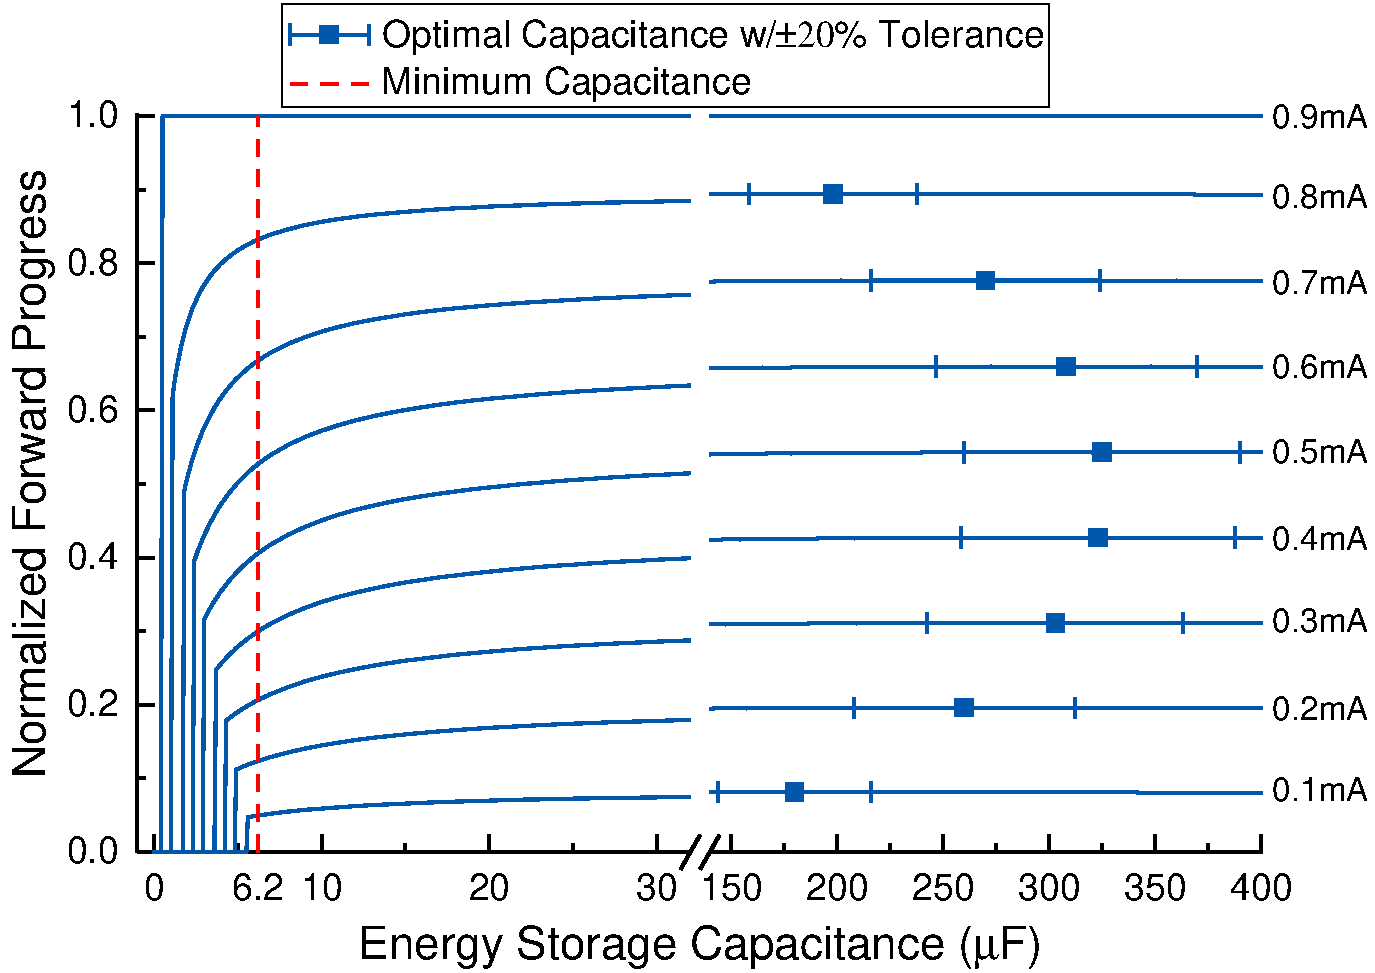
\includegraphics[width=3.2in]{ch3_sizingeffect/figures/StorCCur6Fig} 
  \caption{Forward progress against energy storage capacitance at different levels of constant supply current. Error bars around optimal points denote the impact of typical $\pm$20\% capacitance tolerance. }
  \label{fig:fpwconstcurr}
\end{figure}

\begin{figure}[!t]
  \centering
  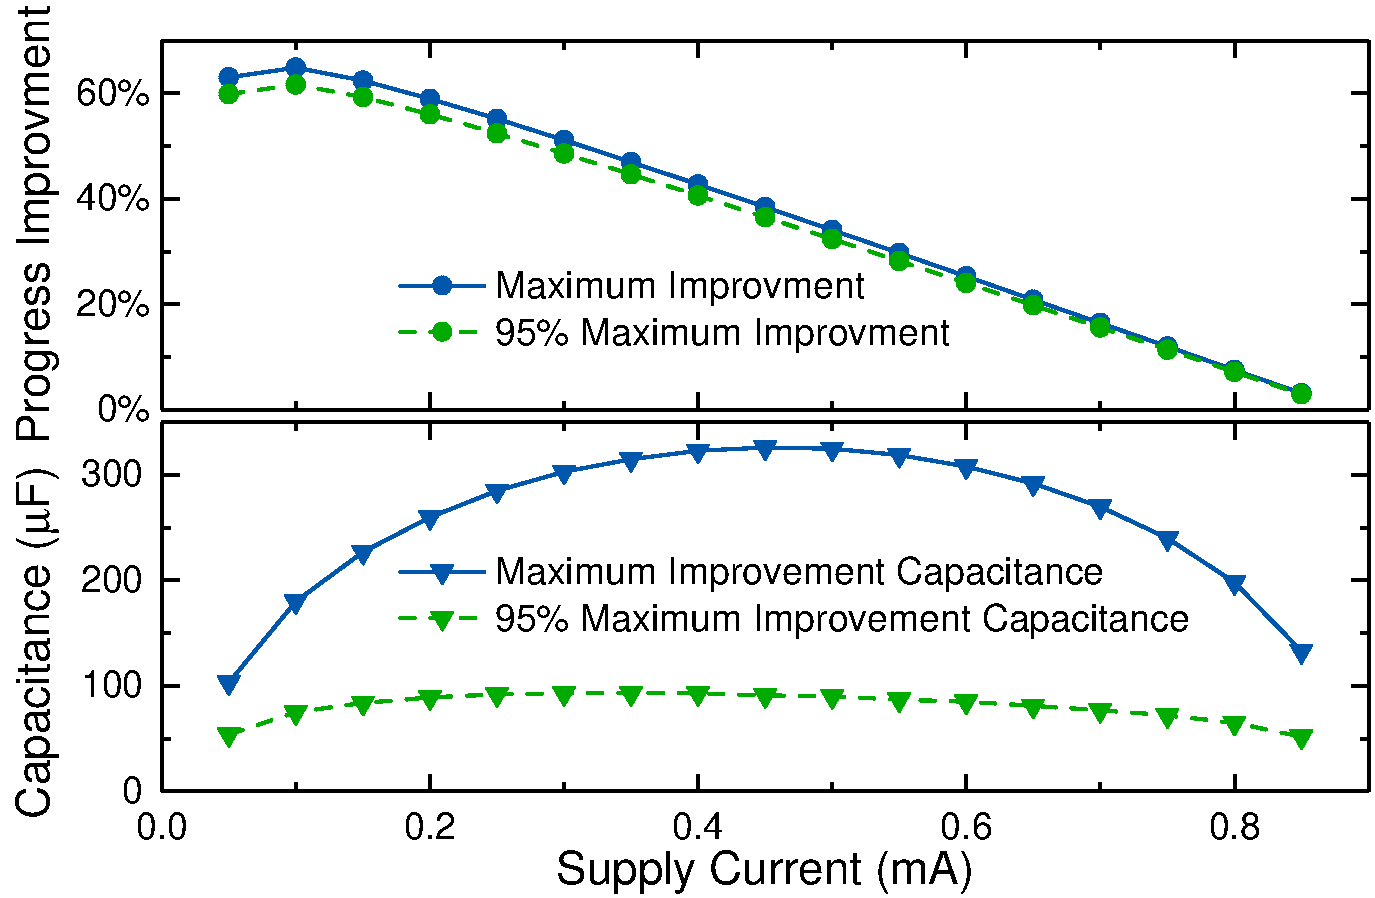
\includegraphics[width=3.2in]{ch3_sizingeffect/figures/StorCCurMax4Fig}
  \caption{Maximum forward progress improvement by sizing energy storage given a spectrum of supply current (normalized by the minimum capacitance case), with the corresponding maximum and sub-maximum (95\% of maximum) capacitance. }
  \label{fig:maxfwp}
\end{figure}

\figurename{~\ref{fig:maxfwp}} shows that an improvement in forward progress of up to 65\%  can be achieved when using the optimal capacitance instead of the minimum. However, it may not be desirable to set the capacitance solely for maximizing forward progress, because there are often trade-offs with other factors including increased interruption periods and dimensions. 
% (explored in Section~\ref{subsec:tradeoff}).
% In real-world energy source conditions, the supply current varies across this spectrum, and hence leads to an overall progress improvement based on its supply distribution. 
% This improvement exists only when the device operates in the Intermittent mode, since the device keeps either inactive in the Off mode or active in the On mode without the need for restoring and saving state. 
% Correspondingly, the optimal energy storage capacity is also plotted against supply current. 
% This optimal capacity exists because of the side effect of capacitor leakage; without capacitor leakage effect, the forward progress would keep approaching the ideal case (as explained in Section~\ref{subsec:formulation}). 
While a large improvement can be delivered with the optimal capacitance, as shown in \figurename{~\ref{fig:maxfwp}}, 95\% of this gain can still be obtained with significantly smaller capacitances (mean 31\% of the optimal value).
For example, reducing from \SI{325}{\micro\farad} to \SI{90}{\micro\farad} gives 95\% of the maximum improvement with a \SI{0.5}{\milli\ampere} supply. 

% in real deployment, storage fixed while current varies, change over a range, we may need to pick a capacity that optimise the majority of energy conditions. 

\subsubsection{Impact of Volatile State Size}

The size of volatile state differs across applications with different amounts of RAM usage, and hence incurs varying time and energy overheads for restore and save operations. We measured time overheads of restore and save operations in the minimum case (64B register data and a 160B stack) and the maximum case (64B register data and a full 2048B RAM) respectively as shown in Table~\ref{tab:ramscale}. As these time overheads are expected to be linear to the state size~\cite{Sliper:2019:ESR:3316781.3317812}, the model can be tuned for various volatile state sizes by linearly scaling the profiled values. 

% In the MCU we explore, volatile state includes CPU registers and SRAM data, which takes 64B and 160-2048B. 

\begin{table}[!t]
    \renewcommand{\arraystretch}{1.2}
    \centering
    \caption{Linear scaling range of volatile state size and restore/save time overheads}
    \label{tab:ramscale}
    \begin{tabular}{|c|cc|}
    \hline
    \textbf{State Size} & \multirow{2}{*}{\textbf{Restore Time}} & \multirow{2}{*}{\textbf{Save Time}}\\
    \textbf{(Registers + SRAM)} & & \\
    \hline
    64B + 160B (lower bound) & \SI{232}{\micro\second} & \SI{208}{\micro\second}\\
    % 64B registers + 160B stack
    64B + 2048B (upper bound) & \SI{2.298}{\milli\second} & \SI{2.274}{\milli\second} \\
    % 64B registers + 2048B RAM
    \hline
    \end{tabular}
\end{table}

An example of this is plotted in \figurename{~\ref{fig:ram}}. The forward progress improvement by sizing energy storage increases with the volatile state size, and the optimal capacitance grows accordingly. The improvement becomes insignificant when the volatile state size is small because the restore and save overheads are already negligible. For example, when the workload uses the least volatile state (the leftmost point), the maximum progress improvement is only 3.6\% although the restore and save overheads are reduced by 93\%. 
% This indicates the more efficiently ICSs save/restore, the more useless this work is. 

\begin{figure}[!t]
    \centering
    \includegraphics[width=3.2in]{ch3_sizingeffect/figures/RSTORAM3Fig}
    \caption{Impact of RAM usage (linear to restore/save overheads) on sizing energy storage with \SI{0.4}{\milli\ampere} current supply. Improvement and reduction are normalized by the minimum capacitance case. }
    \label{fig:ram}
\end{figure}
                 % Sec V
\section{Sizing under Real-World Energy Conditions} \label{sec:c4_demo}

In this section, we model an IPS with a PV energy harvester to explore the energy storage sizing effect in real-world energy conditions, and demonstrate use of the proposed sizing approach. 

\begin{figure}
    \centering
    \includegraphics[width=\columnwidth]{ch4_sizingapproach/figures/solarmodel4}
    \caption{System model of a PV-based IPS.}
    \label{fig:Model}
\end{figure}

\subsection{Simulation Configuration}

We integrate the validated reactive IPS model into a system model with a PV energy-harvesting supply as shown in \fref{fig:Model}. 
The energy storage model and the intermittent load model are as presented in \sref{sec:c3_exploration}. 

We use a converter-less supply circuit where only a Schottky diode is connected to the energy harvester output in order to prevent current backflow. 
The energy source conditions are imported from NREL outdoor solar irradiance data~\cite{stoffel1981nrel} and EnHANTs indoor irradiance data~\cite{6244798}. 
Four sets of light conditions are used to encompass different energy environments. 
To convert irradiance into harvested power, we adopt a PV cell model~\cite{en9050326} which uses the parameters available in common datasheets, so it can easily be reconfigured to suit various devices. 
The output current \nm{I}{o} of the PV cell model can then be described as:
\begin{equation} \label{eq:pvcell}
    \nmm{I}{o} = \frac{G}{\nmm{G}{ref}} \nmm{I}{sc} (1 - (1 - \frac{\nmm{I}{mpp}}{\nmm{I}{sc}}) ^ {\frac{\nmm{V}{o}-\nmm{V}{oc}}{\nmm{V}{mpp} - \nmm{V}{oc}}})
\end{equation}
where \nm{V}{o} is the output voltage of the PV cell, $G$ is the ambient irradiance, \nm{G}{ref} is the reference irradiance (normally \SI{1000}{\watt\per\square\centi\meter}), and \nm{I}{sc}, \nm{V}{oc}, \nm{I}{mpp}, \nm{V}{mpp} are respectively short-circuit current, open-circuit voltage, and the current and voltage at maximum power point (MPP) given the reference irradiance. 
\nm{V}{o} and $G$ are dynamic at run time, while other parameters in this model are constant. 
We refer to Panasonic Amorton glass type solar cells~\cite{solarcell} for PV cell properties as shown in \tref{tab:pvcell}. 
We set four cells in series (with \nm{V}{oc} = 3.56V) to match the operating voltage of the MCU (maximum 3.6V), and model energy harvester sizing by scaling the cell area. 


% A PV panel is an array of PV cells, which amplifies voltage and current output by connecting PV cells in series or parallel. In a PV panel, the open-circuit voltage is proportional to the number of cells in series, and the short-circuit current is proportional to the area of each cell and the number of cells in parallel. 

\begin{table}
    \renewcommand{\arraystretch}{1.2}
    \centering
    \begin{tabular}{|c|c|}
    \hline
    \textbf{Parameter} & \textbf{Value}\\
    \hline
    Open-Circuit Voltage & \SI{0.89}{\volt}/cell\\
    Short-Circuit Current & \SI{14.8}{\milli\ampere\per\square\centi\meter}\\
    Maximum Power Voltage & \SI{0.65}{\volt}/cell\\ 
    Maximum Power Current & \SI{12.1}{\milli\ampere\per\square\centi\meter}\\
    \hline
    \end{tabular}
    \caption{PV cell properties under a \SI{1000}{\watt\per\square\centi\meter}, AM-1.5 light source.}
    \label{tab:pvcell}
\end{table}

Our simulation tool can perform two simulation processes: (a) sort and process the time distribution of environmental conditions, and (b) simulate system state chronologically with a fine-grained time step. 
Process (a) reduces simulation time significantly, e.g. from hours to seconds, but ignores the restore operation after a brownout reset, hence overestimating forward progress, and it overestimates more with smaller capacitance and lower supply current. 
In the following results, \fref{fig:harvstor} comes from Process (a) for fast exploration, and \fref{fig:interruption} and \fref{fig:tradeoff} come from Process (b) for accurate records of interruption periods. 

\subsection{Exploration with Real-World Energy Source Conditions} \label{subsec:harvstor}

% Goal: 
% 1. to show that this model can help designers to find a suitable size of EH to achieve their desired performance;
% 2. to show that sizing energy storage would have different degrees of impact on real deployment depending on the specific energy conditions;
% 3. demonstrate sizing approach. 

In real-world deployments, ambient energy source conditions are dependent on time and location. 
The energy harvester and storage need to be sized to achieve the desired forward progress across the range of expected conditions. 

\subsubsection{Sizing the Energy Harvester}

For the purposes of this exploration, three levels of baseline mean forward progress (\nm{\alpha}{exe}) are set as 0.1, 0.2, and 0.3. 
We use the system model to find the PV panel area that achieves the expected forward progress under the different energy source conditions with minimum energy storage. 
We scale the PV panel area to find that which achieves each baseline \nm{\alpha}{exe}. 
As shown in \fref{fig:harvstor}, the energy harvester sizes that achieve the desired \nm{\alpha}{exe} may span orders of magnitude given different energy source conditions from \SI{}{\square\milli\meter} for outdoor sources ((c) and (d)) to \SI{}{\square\centi\meter} for indoor sources ((a) and (b)).  

\subsubsection{Sizing the Energy Storage}

Having obtained the energy harvester sizes for the baseline forward progress, we then use the modelling approach to size energy storage.
% A table lists the PV panel area to achieve the target \nm{\alpha}{exe} with minimum energy storage capacitance, the optimal capacitance with the forward progress improvement, and the alternative (decreased) PV panel area with the optimal capacitance. 
We analyse the sizing effect of energy storage on forward progress given real-world energy conditions. \fref{fig:harvstor} shows a 7.8-43.3\% improvement in forward progress by sizing energy storage under the given real-world energy conditions and baseline energy harvester sizes. 
It can also be inferred that optimising energy storage can either improve forward progress for a given energy harvester size, or reduce the energy harvester size that achieves the target forward progress. 
Given higher-power energy sources (e.g. Denver 2018 and Hawaii 2018 outdoor solar), increasing the harvester size efficiently improves forward progress with minor dimensional overheads, e.g. tens of \SI{}{\square\milli\meter}; however, given lower-power sources (e.g. EnHANTs Setup~A and Setup~D indoor light), optimising energy storage capacitance can save tens of \SI{}{\square\centi\meter} of PV panel area to achieve the same forward progress.

Also, the progress improvement by sizing energy storage varies accordingly with energy source conditions. 
As mentioned in \cref{chapter:sizingeffect}, this improvement stems from the reduction of restore and save overheads when the supply current is low and the device work in the \textit{Intermittent} mode. 
Thus, the results of EnHANTs Setup~A and Setup~D show a higher progress improvement from sizing energy storage than those of Denver 2018 and Hawaii 2018. 

\begin{figure}
    \centering
    \begin{subfigure}{0.51\columnwidth}
        \centering
        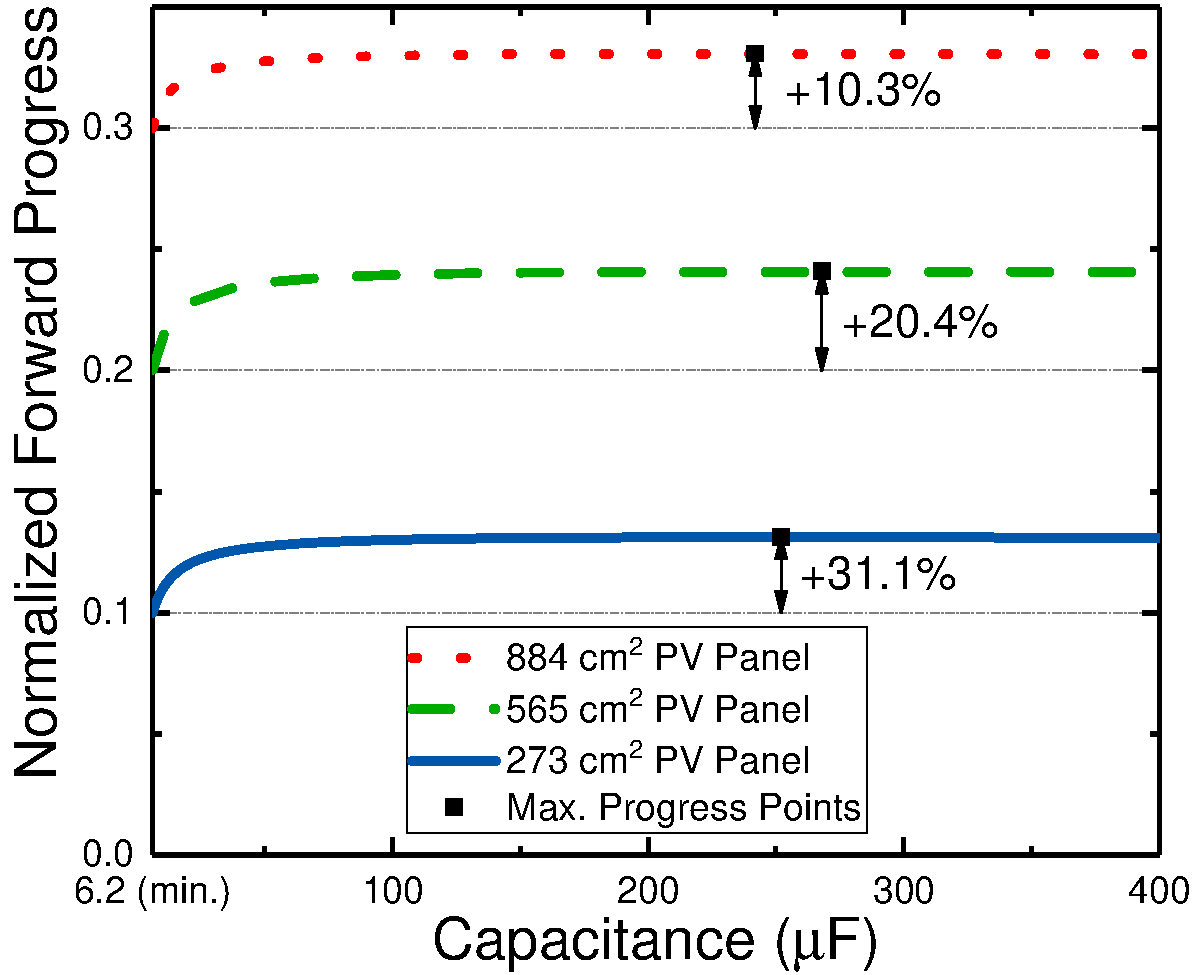
\includegraphics[width=\columnwidth]{ch4_sizingapproach/figures/HarvStorTgFig1}
        \caption{EnHANTs Setup A}
        \label{fig:harvstor1}
    \end{subfigure}
    \begin{subfigure}{0.483\columnwidth}
        \centering
        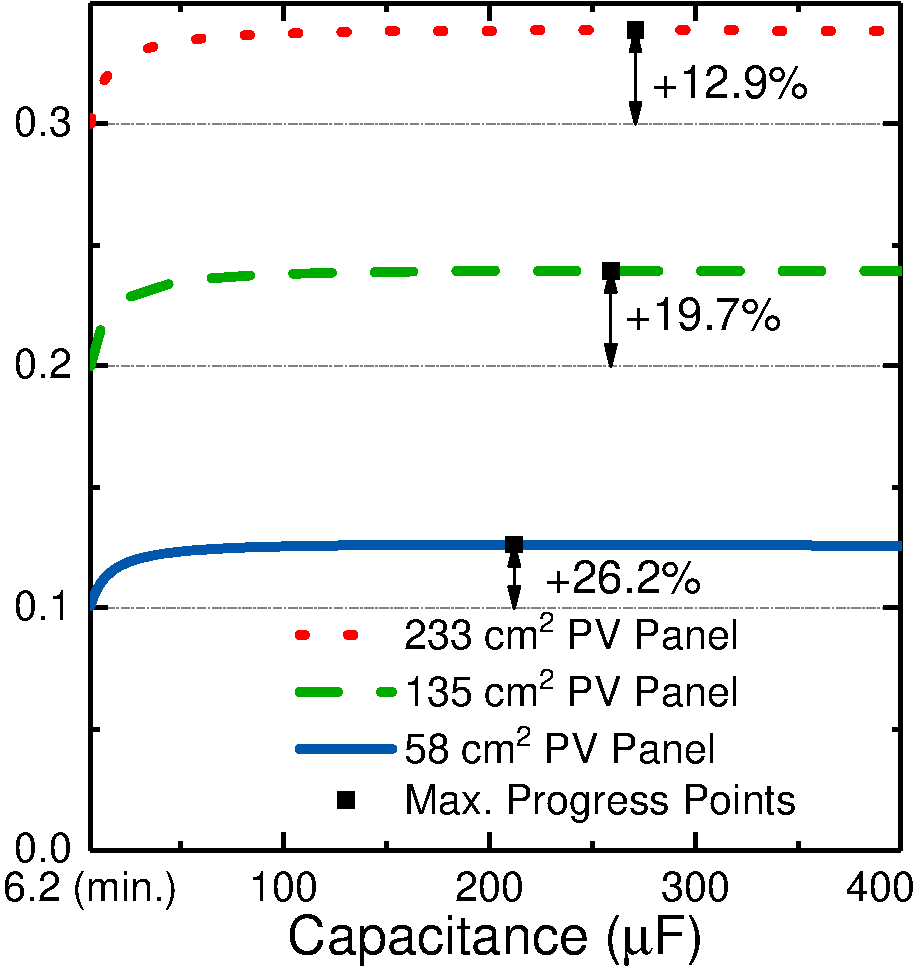
\includegraphics[width=\columnwidth]{ch4_sizingapproach/figures/HarvStorTgFig2}
        \caption{EnHANTs Setup D}
        \label{fig:harvstor2}
    \end{subfigure}
    \hfil
    \begin{subfigure}{0.51\columnwidth}
        \centering
        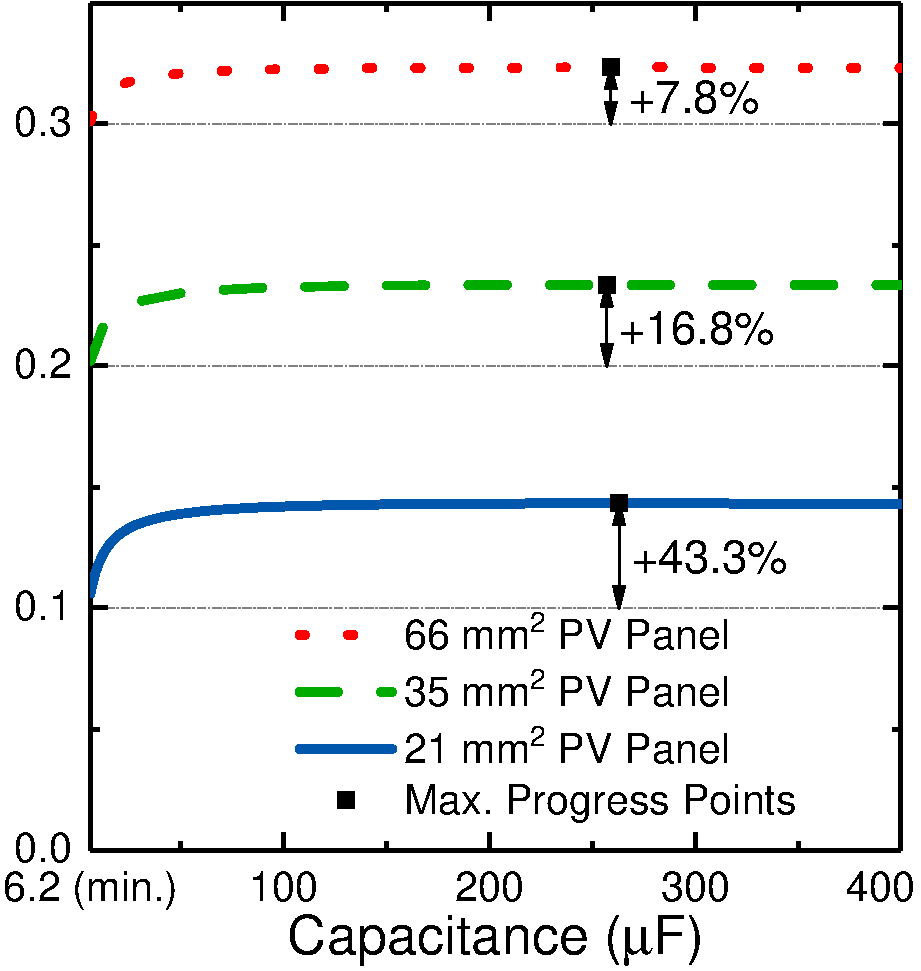
\includegraphics[width=\columnwidth]{ch4_sizingapproach/figures/HarvStorTgFig3}
        \caption{NREL Denver 2018}
        \label{fig:harvstor3}
    \end{subfigure}
    \begin{subfigure}{0.483\columnwidth}
        \centering
        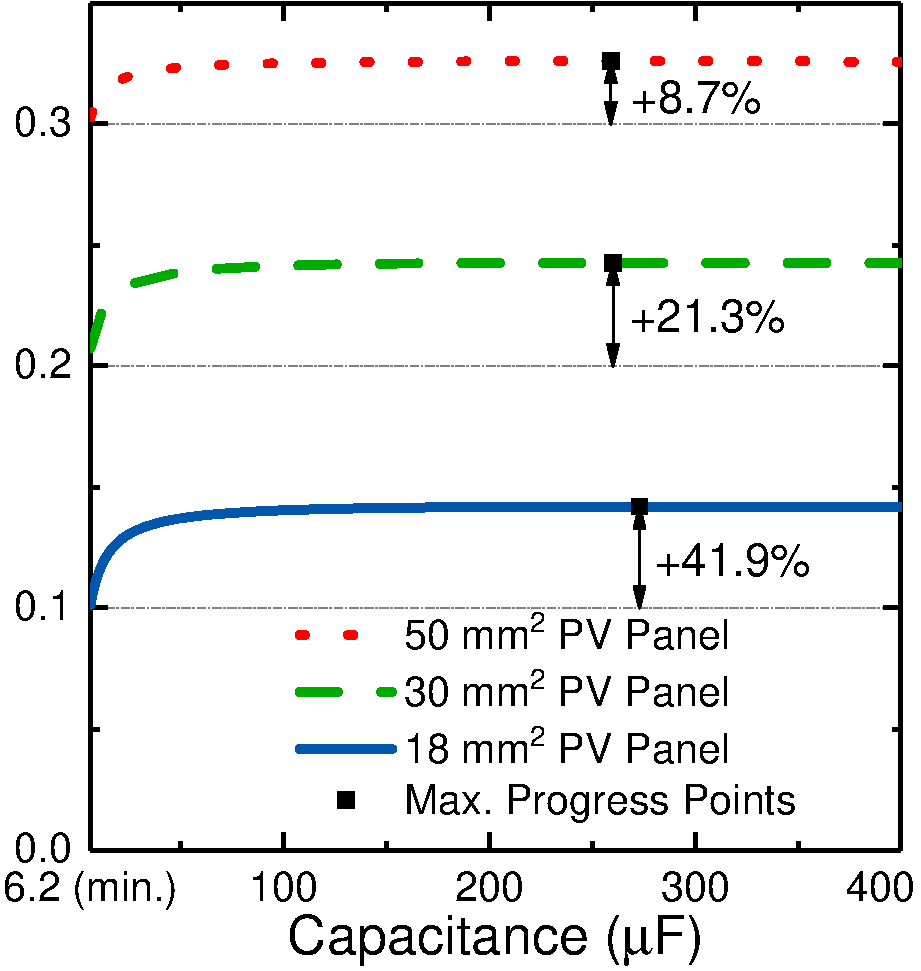
\includegraphics[width=\columnwidth]{ch4_sizingapproach/figures/HarvStorTgFig4}
        \caption{NREL Hawaii 2018}
        \label{fig:harvstor4}
    \end{subfigure}
    \caption{Improvement of average forward progress by sizing energy storage given different PV panel areas under real-world energy source conditions. The model is able to find the PV panel area required for achieving the target mean forward progress. } 
    \label{fig:harvstor}
\end{figure}

The mean forward progress given target \nm{\alpha}{exe} = 0.1 is plotted in \fref{fig:harvstorrange}, with the 60th and 90th time percentiles of forward progress. In all the  above datasets, the energy source is absent and the system is off for around \SI{55}{\percent} of time, so we plot the percentiles from the 60th. The mean progress during the energy-available periods is averaged over the energy-absent periods, so the actual mean forward progress during the energy-available periods is nearly double the annual mean. 

% Absolute improvement are different? Large variations? What other results can I add? 
% The variations of forward progress are significant due to the large variations of energy source conditions, so practical implementation should consider such variation as .
% The improved progress during the energy-available periods is averaged over the energy-absent periods, so the actual amount of improvement when energy is available is higher than the mean. (wrong statement)

\begin{figure}
    \centering
    \begin{subfigure}{0.51\columnwidth}
        \centering
        \includegraphics[width=\columnwidth]{ch4_sizingapproach/figures/HarvStorRan2Fig1}
        \caption{EnHANTs Setup A}
        \label{fig:harvstorrange1}
    \end{subfigure}
    \begin{subfigure}{0.483\columnwidth}
        \centering
        \includegraphics[width=\columnwidth]{ch4_sizingapproach/figures/HarvStorRan2Fig2}
        \caption{EnHANTs Setup D}
        \label{fig:harvstorrange2}
    \end{subfigure}
    \hfil
    \begin{subfigure}{0.51\columnwidth}
        \centering
        \includegraphics[width=\columnwidth]{ch4_sizingapproach/figures/HarvStorRan2Fig3}
        \caption{NREL Denver 2018}
        \label{fig:harvstorrange3}
    \end{subfigure}
    \begin{subfigure}{0.483\columnwidth}
        \centering
        \includegraphics[width=\columnwidth]{ch4_sizingapproach/figures/HarvStorRan2Fig4}
        \caption{NREL Hawaii 2018}
        \label{fig:harvstorrange4}
    \end{subfigure}
    \caption{Time percentiles of forward progress by sizing energy storage with target \nm{\alpha}{exe} = 0.1 and the corresponding PV panel area listed in \fref{fig:harvstor}. The percentiles start from the 60th as the system is off for around \SI{55}{\percent} of time due to insufficient energy source. }
    \label{fig:harvstorrange}
\end{figure}

\subsubsection{Interruption Period} \label{subsubsec:intper}
Besides forward progress, we also explore how the capacitance can change the interruption periods. 
When interrupted by insufficient power supply, an IPS enters an interruption period where it saves its volatile state, waits for supply voltage to recover, and restores the state to resume execution, without making any forward progress. 
Applications that require frequent sensing may be negatively affected by long interruption periods. 
We measure an interruption period as \textit{the period between two successive execution periods}, e.g. a consecutive `SLR' period in \fref{fig:operatingCycle} forms an interruption period. 
We record all the interruption periods during a one-year simulation with \SIrange{10}{50}{\micro\farad} capacitors, the Denver 2018 dataset, and an \SI{80}{\square\milli\meter} PV panel. 
\fref{fig:interruption} presents the distribution of all the interruption periods. 
With increased energy storage, the interruption period is prolonged. 
For example, the 90th percentile of interruption periods increases from \SI{32.2}{\milli\second} at \SI{10}{\micro\farad} to \SI{123.4}{\milli\second} at \SI{50}{\micro\farad} at an approximate rate of \SI{23}{\milli\second} per \SI{10}{\micro\farad}. 
% The majority of the interruption periods are within \SI{200}{\milli\second}. 
Facilitated by the simulator, developers are enabled to estimate whether the distribution of interruption periods meet their application requirement. 

% Whether and how much this would affect  Time-sensitive applications may care 
% the total number of interruptions is reduced,


\begin{figure}
    \centering
    \includegraphics[width=\columnwidth]{ch4_sizingapproach/figures/IntPeriodOrdFig}
    \caption{Distribution of interruption periods. }
    \label{fig:interruption}
\end{figure}

\subsection{Trading Forward Progress, Dimensions, and Interruption Period} \label{subsec:tradeoff}

Although increasing energy storage capacitance improves forward progress, larger capacitance increases both dimensions and interruption periods. 
We evaluate the overheads of increased capacitor dimensions and interruption periods, and then trade them off against forward progress using a cost function to suggest an optimal capacitance value. 

\subsubsection{Metric of Dimensions}

The overhead of capacitor dimensions is evaluated by characteristics of off-the-shelf tantalum capacitors. 
We narrow down the range of sample capacitors within a set of characteristics: low-profile, 10V rated voltage, and surface-mount package, and select six series of capacitors\footnote{The series of capacitor considered were: AVX TAJ, AVX TACmicrochip, AVX F92, Vishay 572D, Vishay 591D, and Vishay 592D.}. 
The volume and capacitance of these devices are plotted in \fref{fig:capvol}. 
We use the regression of these data to approximate a capacitance-volume relationship.
% ~\cite{tancap1, tancap2, tancap3, tancap4, tancap5, tancap6}
% Among the common capacitor chemistries with \textmu F to mF capacitance, tantalum capacitors manifest low leakage 

\begin{figure}
    \centering
    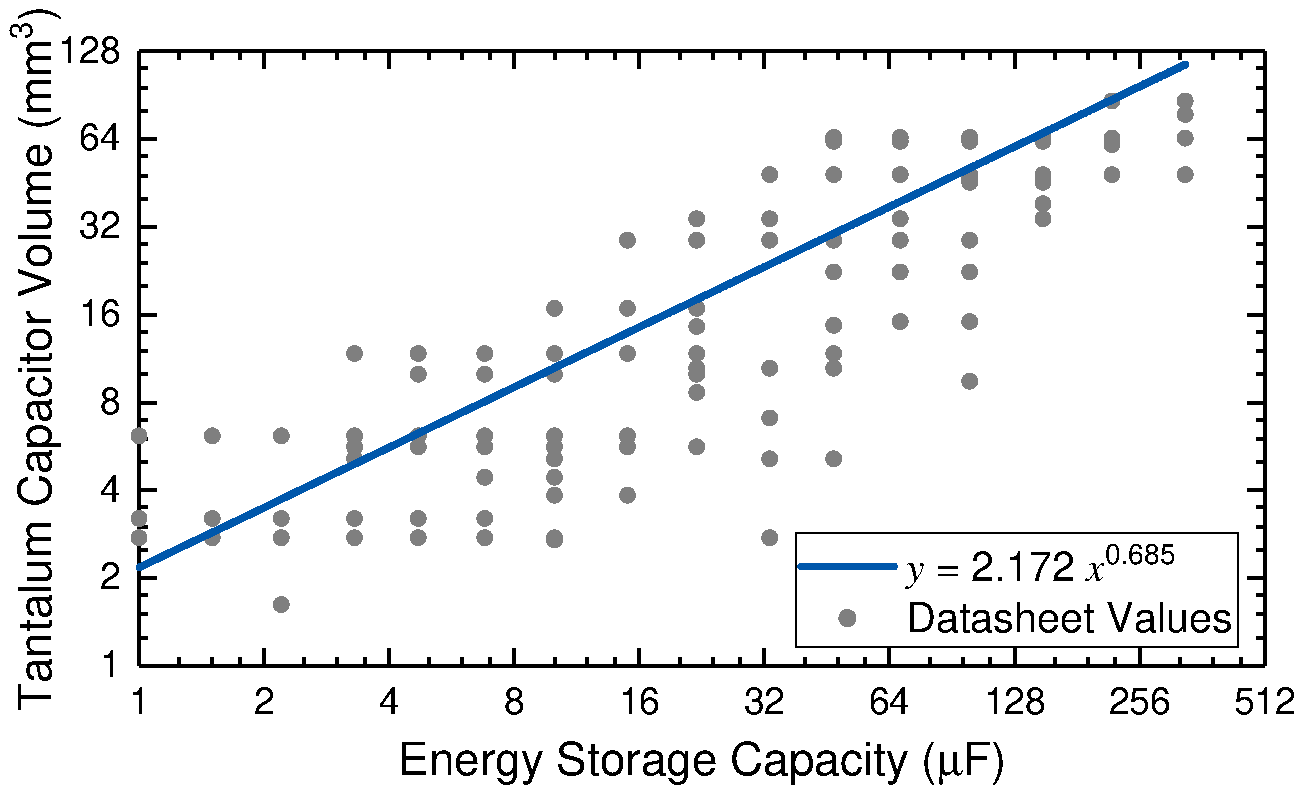
\includegraphics[width=\columnwidth]{ch4_sizingapproach/figures/CapVol2Fig2}
    \caption{Tantalum capacitor volume against capacitance for the six series of capacitors analysed. }
    \label{fig:capvol}
\end{figure}

\subsubsection{Metric of Interruption Periods} \label{subsubsec:metricintper}

% Definition/Measurement of interruption periods. recharging ability? Considering leakage?
% why interruption periods is important, why we consider it.

% , i.e. the period that does not make forward progress. The total interruption periods should be opposite to forward progress. 
Applications may have various requirements on interruption periods. 
To demonstrate the usage of our sizing approach, we consider a designer requests the 90th percentile of all interruption periods as an example metric of interruption periods, denoted as \nm{T}{int}. 
This metric indicates 90\% of interruption periods are shorter than \nm{T}{int}. 
This metric can be adapted for particular application requirements. 
% In We assume that $T_{interrupt}$ is preferable to be short for general application. 

\subsubsection{Cost Function}

From the previous observations (\fref{fig:maxfwp}) we can see that achieving the optimal progress improvement costs much more capacitance (mean 3.2$\times$) than to achieve 95\% improvement. 
A trade-off is necessary to improve forward progress while restricting the overheads of increased capacitor volume and interruption periods. 
This involves a problem of multi-criteria decision making~\cite{triantaphyllou2000multi}, which is outside the scope of this work. 
Nevertheless, we provide a cost function in (\ref{eq:tradeoff}) as an example to illustrate how these three factors could be traded-off, but designers are expected to customise a cost function with parameters of importance to specific application requirements. 
Note that the function (\ref{eq:tradeoff}) is to be maximised to find the recommended capacitance. 
\begin{equation}
    f = \frac{\nmm{\alpha}{exe}}{\nmm{k}{1}} - \left(\frac{\nmm{v}{cap}}{\nmm{k}{2}}\right) ^ {2} - \left(\frac{\nmm{T}{int}}{\nmm{k}{3}}\right) ^ {2} 
    \label{eq:tradeoff}
\end{equation}
\nm{\alpha}{exe} denotes normalised forward progress, \nm{v}{cap} denotes capacitor volume, and \nm{T}{int} denotes application interruption periods as mentioned in \sref{subsubsec:metricintper}. 
\nm{\alpha}{exe}, \nm{v}{cap}, and \nm{T}{int} can be generated from the simulation tool given $C$ as an input. 
\nm{k}{1}, \nm{k}{2}, and \nm{k}{3} are coefficients for normalising each metric, and they are empirically determined according to applications. 
In this example, the undesirable parameters are expressed as quadratic and negative terms to give an increasing cost to higher values. 
While only three parameters are considered here, others (such as the energy harvester size) could be included for a system-wise sizing scenario.
As an example to demonstrate its usage, we arbitrarily configure the function by setting \nm{k}{1} = 0.2, \nm{k}{2} = \SI{200}{\cubic\milli\meter}, and \nm{k}{3} = \SI{500}{\milli\second}. 
%, i.e.:
%\begin{equation}
%    f = \frac{\nmm{\alpha}{exe}}{0.2} - (\frac{\nmm{v}{cap}}{200}) ^ {2} - T_{recharge} ^ {2} 
%    \label{eq:tradeoffuse}
%\end{equation}
% where \nm{v}{cap} is in \SI{}{\cubic\milli\meter} and $T_{recharge}$ is in second. Here, $\frac{1}{\nmm{k}{1}} / \frac{1}{\nmm{k}{2}}$ equals 1000, but this does not mean that forward progress is 1000 times more important than capacitor volume.

\subsubsection{Results}

The effect of the trade-off is plotted in \fref{fig:tradeoff} using the Denver 2018 energy source dataset. 
Compared to the capacitor size that solely maximises forward progress, on average, an appropriately-sized capacitor achieves 93\% of the maximum forward progress, while saving 83\% of capacitor volume and 91\% of interruption periods. 
This also demonstrates the efficacy of the cost function and the chosen coefficients. 
Compared to the minimum storage case, the appropriately-sized capacitor improves forward progress by 12-124\% with energy storage increased from \SI{6.2}{\micro\farad} to \SI{30}{\micro\farad}.

\begin{figure}
    \centering
    \includegraphics[width=\columnwidth]{ch4_sizingapproach/figures/Tradeoff3Fig}
    \caption{The sizing approach trades off forward progress, capacitor volume, and interruption periods. The results are plotted against a range of PV panel area, given Denver 2018 energy source dataset. }
    \label{fig:tradeoff}
\end{figure}

As shown in \fref{fig:capvol}, the closest available capacitance that satisfies the \SI{6.2}{\micro\farad} minimum capacitance is \SI{6.8}{\micro\farad}, whereas the closest available capacitance to the appropriate \SI{30}{\micro\farad} is \SI{33}{\micro\farad}. 
The minimum volumes of \SI{6.8}{\micro\farad} and \SI{33}{\micro\farad} capacitors are both \SI{2.75}{\cubic\milli\meter}, which means using the appropriate capacitance, instead of the minimum one, may not incur dimensional overhead. 
% For \SI{47}{\micro\farad}, the absolute volume (\SI{5.12}{\cubic\milli\meter}) is insignificant compared to the device as a whole, e.g. an MSP430FR6989 MCU chip alone occupies \SI{274.4}{\cubic\milli\meter} (14 $\times$ 14 $\times$ 1.4). 
The regressed volume of the above two capacitance values are \SI{8.1}{\cubic\milli\meter} and \SI{23.8}{\cubic\milli\meter} respectively. 
However, the selection of capacitors can be dependent on factors other than physical volume, such as reliability, operation temperature, and more specific application needs. 
These factors can also be added into the cost function if necessary. 
% Again, such a volume scale is still insignificant in a whole device. 

                  % Sec VII

%%%%%%%%%%%%%%%%%%%%%%%%%%%%%%%%%%%%%%%%%%%%%%%%%%%%%%%%%%
%%% Section VIII: Conclusion
%%%%%%%%%%%%%%%%%%%%%%%%%%%%%%%%%%%%%%%%%%%%%%%%%%%%%%%%%%

\section{Conclusions} \label{section:conclusion}

% We explored the relationship between forward progress and energy storage capacitance in intermittent computing through a theoretical model.

% In this paper, we presented a model of reactive ICSs that accurately estimates forward progress. 
% Using this model, we explored the sizing effect of energy storage on forward progress with respect to supply current and volatile state size, showing up to \SI{64.9}{\percent} progress improvement under constant current supply and \SIrange{7.8}{43.3}{\percent} improvement on annual mean forward progress 
% under various real-world energy conditions. 

While conventional ICSs have used minimal levels of capacitance, this paper has shown that increasing the amount of energy storage can improve system performance by up to 65\% with a constant current supply and 43\% with real-world PV sources. The work includes a simulation tool which is available to download, enabling researchers to experiment with energy storage sizes to optimize ICS designs. A cost function can be incorporated, allowing various aspects of system performance to be traded-off. Our conclusion is that energy storage should be carefully designed, rather than minimized or indiscriminately picked, to efficiently operate ICSs.
%\color{blue}
%\todo{Alex to update this after other parts completed/queries resolved.}In this paper, we explored the energy storage sizing effect on ICS forward progress, concluding that adding a relatively small amount of energy storage can significantly improve forward progress. 
%We proposed an approach for sizing energy storage, which improves forward progress with insignificant overheads on capacitor volume and interruption periods. 
% We integrated the model into a PV-based ICS framework to demonstrate the sizing approach, where results show that the suggested energy storage capacitance achieves \SI{98.3}{\percent} of the maximum forward progress while saving \SI{71.7}{\percent} capacitor volume and \SI{83.8}{\percent} interruption periods. 
% We validated the reactive intermittent computing model, which demonstrates only \SI{0.5}{\percent} mean absolute percentage error on forward progress compared to the experimentally measured values.
% Experimental results also showed that a reasonably sized \SI{43}{\micro\farad} capacitor improves forward progress by up to \SI{55.2}{\percent} and \SI{30.4}{\percent} compared to a theoretical minimum \SI{6.2}{\micro\farad} one and an on-board \SI{10}{\micro\farad} one across various levels of supply current. 
%We believe that the problem of frequent power interruptions in energy-harvesting supply can be easily alleviated by using an appropriately-sized capacitor. 
% Instead, the design of energy storage plays a significant role in practical deployment. 
%\color{black}


% An example of a floating figure using the graphicx package.
% Note that \label must occur AFTER (or within) \caption.
% For figures, \caption should occur after the \includegraphics.
% Note that IEEEtran v1.7 and later has special internal code that
% is designed to preserve the operation of \label within \caption
% even when the captionsoff option is in effect. However, because
% of issues like this, it may be the safest practice to put all your
% \label just after \caption rather than within \caption{}.
%
% Reminder: the "draftcls" or "draftclsnofoot", not "draft", class
% option should be used if it is desired that the figures are to be
% displayed while in draft mode.
%

% Note that the IEEE typically puts floats only at the top, even when this
% results in a large percentage of a column being occupied by floats.


% An example of a double column floating figure using two subfigures.
% (The subfig.sty package must be loaded for this to work.)
% The subfigure \label commands are set within each subfloat command,
% and the \label for the overall figure must come after \caption.
% \hfil is used as a separator to get equal spacing.
% Watch out that the combined width of all the subfigures on a 
% line do not exceed the text width or a line break will occur.
%
%\begin{figure*}[!t]
%\centering
%\subfloat[Case I]{\includegraphics[width=2.5in]{box}%
%\label{fig_first_case}}
%\hfil
%\subfloat[Case II]{\includegraphics[width=2.5in]{box}%
%\label{fig_second_case}}
%\caption{Simulation results for the network.}
%\label{fig_sim}
%\end{figure*}
%
% Note that often IEEE papers with subfigures do not employ subfigure
% captions (using the optional argument to \subfloat[]), but instead will
% reference/describe all of them (a), (b), etc., within the main caption.
% Be aware that for subfig.sty to generate the (a), (b), etc., subfigure
% labels, the optional argument to \subfloat must be present. If a
% subcaption is not desired, just leave its contents blank,
% e.g., \subfloat[].


% An example of a floating table. Note that, for IEEE style tables, the
% \caption command should come BEFORE the table and, given that table
% captions serve much like titles, are usually capitalized except for words
% such as a, an, and, as, at, but, by, for, in, nor, of, on, or, the, to
% and up, which are usually not capitalized unless they are the first or
% last word of the caption. Table text will default to \footnotesize as
% the IEEE normally uses this smaller font for tables.
% The \label must come after \caption as always.


% Note that the IEEE does not put floats in the very first column
% - or typically anywhere on the first page for that matter. Also,
% in-text middle ("here") positioning is typically not used, but it
% is allowed and encouraged for Computer Society conferences (but
% not Computer Society journals). Most IEEE journals/conferences use
% top floats exclusively. 
% Note that, LaTeX2e, unlike IEEE journals/conferences, places
% footnotes above bottom floats. This can be corrected via the
% \fnbelowfloat command of the stfloats package.

% if have a single appendix:
% \appendix[Calculation Breakdown of Differential Analysis]

% Haven't decided whether to attach this or not. 

% \section*{test}
% text goes.
% \section*{test2}

% or
%\appendix  % for no appendix heading
% do not use \section anymore after \appendix, only \section*
% is possibly needed

% use appendices with more than one appendix
% then use \section to start each appendix
% you must declare a \section before using any
% \subsection or using \label (\appendices by itself
% starts a section numbered zero.)
%

% \appendices
% \section{Proof of the First Zonklar Equation}
% Appendix one text goes here.

% use section* for acknowledgment
% \section*{Acknowledgment}


% The authors would like to thank...


% Can use something like this to put references on a page
% by themselves when using endfloat and the captionsoff option.
\ifCLASSOPTIONcaptionsoff
  \newpage
\fi



% trigger a \newpage just before the given reference
% number - used to balance the columns on the last page
% adjust value as needed - may need to be readjusted if
% the document is modified later
%\IEEEtriggeratref{8}
% The "triggered" command can be changed if desired:
%\IEEEtriggercmd{\enlargethispage{-5in}}

% references section

% can use a bibliography generated by BibTeX as a .bbl file
% BibTeX documentation can be easily obtained at:
% http://mirror.ctan.org/biblio/bibtex/contrib/doc/
% The IEEEtran BibTeX style support page is at:
% http://www.michaelshell.org/tex/ieeetran/bibtex/
\bibliographystyle{IEEEtran}
\IEEEtriggeratref{27}
\bibliography{ref}
%
% <OR> manually copy in the resultant .bbl file
% set second argument of \begin to the number of references
% (used to reserve space for the reference number labels box)
% \begin{thebibliography}{1}

% \bibitem{IEEEhowto:kopka}
% H.~Kopka and P.~W. Daly, \emph{A Guide to \LaTeX}, 3rd~ed.\hskip 1em plus
%   0.5em minus 0.4em\relax Harlow, England: Addison-Wesley, 1999.

% \end{thebibliography}

% biography section
% 
% If you have an EPS/PDF photo (graphicx package needed) extra braces are
% needed around the contents of the optional argument to biography to prevent
% the LaTeX parser from getting confused when it sees the complicated
% \includegraphics command within an optional argument. (You could create
% your own custom macro containing the \includegraphics command to make things
% simpler here.)
%\begin{IEEEbiography}[{\includegraphics[width=1in,height=1.25in,clip,keepaspectratio]{mshell}}]{Michael Shell}
% or if you just want to reserve a space for a photo:

\vspace{-6\baselineskip}

\begin{IEEEbiography}[{\includegraphics[width=1in,height=1.25in,clip,keepaspectratio]{jiezhan.jpeg}}]{Jie Zhan}
received the B.Eng. degree in electrical engineering from Xiamen University, China, in 2017. He is currently pursuing a Ph.D. in electronic engineering with the School of Electronics and Computer Science, University of Southampton. His research is focused on efficient intermittent computing for batteryless energy-harvesting devices
\end{IEEEbiography}

\vspace{-6\baselineskip}

\begin{IEEEbiography}[{\includegraphics[width=1in,height=1.25in,clip,keepaspectratio]{geoff_merrett_journalbio.jpg}}]{Geoff V. Merrett}

(GSM'06-M'09-SM’19) received the B.Eng. (Hons) and Ph.D. degrees from the University of Southampton, U.K., in 2004 and 2008, respectively. He currently holds a Personal Chair in Electronic and Software Systems at the School of Electronics and Computer Science, University of Southampton, U.K., where he is Head of the Centre for Internet of Things and Pervasive Systems.

Prior to becoming a Professor in 2019, he was a Lecturer and Associate Professor at Southampton from 2009 and 2014 respectively. He is Co-Director of the Arm-ECS Research Centre, an award winning collaboration between the university and Arm Research, Cambridge. His current research interests are in energy management of mobile/embedded systems and self-powered devices, and he has published over 200 journal and conference articles on these topics.
\end{IEEEbiography}
% short bio
% (GSM’06-M’09-SM’19) is Professor of Electronic and Software Systems at the University of Southampton, U.K., where he previously received the B.Eng. (Hons) and Ph.D. degrees in 2004 and 2008, respectively. 
% He is co-director of the Arm-ECS Research Centre, an award winning collaboration between the university and Arm Research, Cambridge. 
% His current research interests are in energy management of mobile/embedded systems and self-powered devices, and he has published over 200 journal and conference articles on these topics.

% additional
% Prof. Merrett was co-editor of the book "Many-Core Computing: Hardware and Software" (IET, 2019), General Chair of EWME 2016 and ENSsys 2013-15, and an Associate Editor for IET CDT and MDPI Sensors. He is a Member of the IET, and a Fellow of the HEA.

\vspace{-6\baselineskip}

\begin{IEEEbiography}[{\includegraphics[width=1in,height=1.25in,clip,keepaspectratio]{alex_weddell_journalbio.jpeg}}]{Alex S. Weddell}
(GSM’06-M’10) received the M.Eng. degree (1st class honors) and Ph.D. in electronic engineering from the University of Southampton, U.K., in 2005 and 2010. His main research focus is in the areas of energy harvesting and energy management for future Internet of Things devices.
He has over 15 years’ experience in energy harvesting systems, and has published over 65 papers in the area. 
He is now a Lecturer at the University of Southampton, involved with three projects funded by EPSRC, EU Horizon 2020 and Clean Sky 2.
\end{IEEEbiography}

% insert where needed to balance the two columns on the last page with
% biographies
%\newpage

% You can push biographies down or up by placing
% a \vfill before or after them. The appropriate
% use of \vfill depends on what kind of text is
% on the last page and whether or not the columns
% are being equalized.

%\vfill

% Can be used to pull up biographies so that the bottom of the last one
% is flush with the other column.
%\enlargethispage{-5in}

% \todos

\end{document}